\documentclass[11pt,a4paper]{article}

\usepackage[utf8]{inputenc}
\usepackage[T1]{fontenc}
\usepackage[english]{babel}
\usepackage{lmodern}
\usepackage{amsmath,amssymb,mathtools,array,booktabs,longtable,tabularx,makecell}
\usepackage{geometry}
\geometry{margin=0.9in}
\usepackage{fancyhdr}
\usepackage{titlesec}
\usepackage{enumitem}
\usepackage{tikz}
\usetikzlibrary{calc,intersections}
\usepackage{pdflscape}
\usepackage{microtype}

\pagestyle{fancy}
\fancyhf{}
\fancyhead[C]{\small Cayley --- Collected Mathematical Papers, Vol. VIII (pp. 367--416)}
\fancyfoot[C]{\thepage}
\renewcommand{\headrulewidth}{0.4pt}

\titleformat{\section}{\large\scshape\centering}{}{0em}{}
\titleformat{\subsection}{\normalsize\bfseries\centering}{}{0em}{}
\setlength{\parindent}{1.3em}
\setlength{\parskip}{0.22em}
\allowdisplaybreaks
\setcounter{secnumdepth}{0}

\newcommand{\sourcepage}[2]{\par\smallskip\noindent\textit{[Printed p.~#1; source PDF p.~#2.]}\par\smallskip}
\newcommand{\pagemarker}[3]{\par\bigskip\noindent\textit{p.~#1 [#2; source PDF p.~#3]}\par\smallskip}
\newcommand{\articlenote}[1]{\begin{center}\small\textit{#1}\end{center}}
\newcommand{\dash}{\text{---}}
\newcommand{\half}{\tfrac12}
\newcommand{\third}{\tfrac13}
\newcommand{\quarter}{\tfrac14}
\newcommand{\sixth}{\tfrac16}
\newcommand{\V}[1]{\sqrt{#1}}
\newcommand{\ddotscell}{\multicolumn{1}{c}{$\cdots$}}
\newcommand{\dd}{\,d}
\newcommand{\Det}{\operatorname{Det}}
\newcommand{\sech}{\operatorname{sech}}
\newcommand{\eps}{\varepsilon}

\begin{document}
\sourcepage{367}{431}
\begin{center}
{\large\bfseries 521. ON DR. WIENER'S MODEL OF A CUBIC SURFACE}\\
\smallskip
{\large\bfseries WITH 27 REAL LINES; AND ON THE CONSTRUCTION OF A DOUBLE-SIXER.}
\end{center}

The model is a solid figure bounded by portions of the faces of the cube, and
by a portion of the cubic surface, being a surface with three apertures, the collocation
of which is not easily explained.

To determine the construction I measured, on the faces of the cube, the coordinates
of the two extremities of each of the twelve lines; these were measured in tenths
of an inch (taking account of the half division, or twentieth of an inch), and the
resulting numbers divided by 16 to reduce them to the before-mentioned unit of
$1.6$ inches. These reduced values are shewn in the table: knowing then the
coordinates of two points on each line, the equations of the several lines became
calculable; the true theoretical form of these results---viz. the form which, but for
errors of the model, or of the measurement, they would have assumed---is
\[
\begin{array}{rcl@{\qquad}rcl}
b_1, & x=B_1z+D,       & y=B_1'z+D',\\
b_2, & x=0,            & z=1,\\
b_3, & x=B_3(z+\beta_3), & y=B_3'(z+\beta_3),\\
b_4, & x=B_4(z+\beta_4), & y=B_4'(z+\beta_4),\\
b_5, & y=0,            & z=-1,\\
b_6, & x=B_6(z+\beta_6), & y=B_6'(z+\beta_6),\\[2mm]
a_1, & x=0,            & y=0,\\
a_2, & x=A_2z+C_2,     & y=A_2'(z-1),\\
a_3, & x=A_3(z+1),     & y=A_3'(z-1),\\
a_4, & x=A_4(z+1),     & y=A_4'(z-1),\\
a_5, & x=A_5(z+1),     & y=A_5'z+C_5',\\
a_6, & x=A_6(z+1),     & y=A_6'(z-1);
\end{array}
\]
but in consequence of such errors, the results are not accurately of the form in
question.

The faces of the cube being as in the diagram:
\[
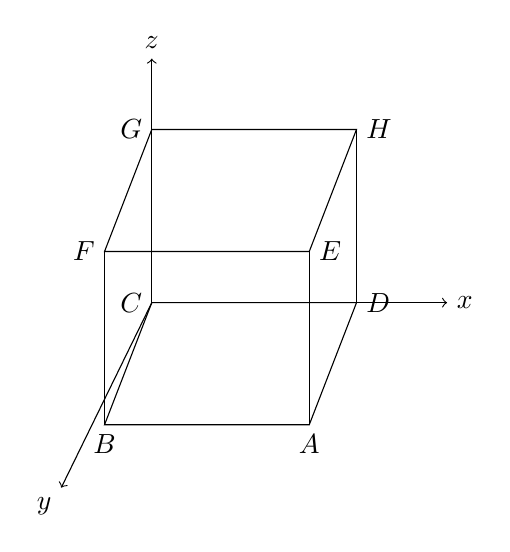
\begin{tikzpicture}[scale=1.0,baseline=(current bounding box.center)]
  \coordinate (B) at (0,0);
  \coordinate (A) at (2.6,0);
  \coordinate (D) at (3.2,1.55);
  \coordinate (C) at (0.6,1.55);
  \coordinate (F) at (0,2.2);
  \coordinate (E) at (2.6,2.2);
  \coordinate (H) at (3.2,3.75);
  \coordinate (G) at (0.6,3.75);
  \draw (B)--(A)--(D)--(C)--cycle;
  \draw (F)--(E)--(H)--(G)--cycle;
  \draw (A)--(E) (B)--(F) (C)--(G) (D)--(H);
  \draw[->] (C)--(0.6,4.65) node[above] {$z$};
  \draw[->] (C)--(4.35,1.55) node[right] {$x$};
  \draw[->] (C)--(-0.55,-0.8) node[below left] {$y$};
  \foreach \p/\pos in {A/below,B/below,C/left,D/right,E/right,F/left,G/left,H/right}
    \node[\pos] at (\p) {$\p$};
\end{tikzpicture}
\]
the Table is as follows.

\sourcepage{368}{432}
\begin{landscape}
\small
\begin{longtable}{>{\raggedright\arraybackslash}p{0.09\linewidth}
                  >{\raggedright\arraybackslash}p{0.18\linewidth}
                  >{\raggedright\arraybackslash}p{0.18\linewidth}
                  >{\raggedright\arraybackslash}p{0.18\linewidth}
                  >{\raggedright\arraybackslash}p{0.18\linewidth}}
\caption*{Equations calculated from the measurements of the model, with endpoint data on the faces of the cube.}\\
\toprule
Line & Calculated equation & First face data & Second face data & Additional face data\\
\midrule
$a_1$ & $x=0,\ y=0$ & $ABCD:\ z=-5.688$ & $EFGH:\ z=+5.688$ & \\
$a_2$ & $x=-0.780z-0.187,\ y=-0.423z+0.406$ & $ABCD:\ x=4.250,\ y=0$ & $EFGH:\ x=-4.625,\ y=0$ & \\
$a_3$ & $x=-0.654z-0.656,\ y=-0.588z+0.531$ & $ABCD:\ x=3.062,\ y=3.875$ & $EFGH:\ x=-4.375,\ y=-2.812$ & \\
$a_4$ & $x=-2.912z-2.959,\ y=-0.736z+0.752$ & $CDGH:\ z=0.9375,\ y=-0.0625$ & $AEDH:\ z=-2.969,\ y=2.937$ & \\
$a_5$ & $x=1.024z+1.014,\ y=-1.049z-0.277$ & $ABCD:\ x=-4.812,\ y=5.688$ & $AEDH:\ y=-5.063,\ z=4.562$ & \\
$a_6$ & $x=-0.264z-0.187,\ y=-0.104z+0.219$ & $ABCD:\ x=-1.313,\ y=-0.8125$ & $EFGH:\ x=1.687,\ y=-0.375$ & \\
$b_1$ & $x=-1.611z+0.151,\ y=-1.438z-0.288$ & $CDGH:\ y=5.500,\ z=-3.625$ & $AEDH:\ y=-4.656,\ z=3.437$ & \\
$b_2$ & $x=0,\ z=-1$ & $AEBF:\ x=0$ & $BCFG:\ x=0$ & \\
$b_3$ & $x=-1.352z-0.685,\ y=-2.034z-0.984$ & $AEBF:\ z=3.750,\ y=-3.281$ & $BCFG:\ x=-3.812,\ z=2.313$ & \\
$b_4$ & $x=-0.753z-0.0315,\ y=-0.500z-0.0315$ & $ABCD:\ x=4.250,\ y=2.812$ & $EFGH:\ x=-4.313,\ y=-2.875$ & \\
$b_5$ & $y=0,\ z=1$ & $CDGH:\ x=1,\ y=0$ & $AEDH:\ y=0$ & \\
$b_6$ & $x=1.123z-0.702,\ y=-1.123z+0.702$ & $AEBF:\ x=-5.688,\ z=-4.438$ & $BCFG:\ y=0$ & $AEDH:\ y=-5.688$\\
\bottomrule
\end{longtable}
\end{landscape}

I hence calculate the intersections: considering any two lines which ought to
intersect, then projecting on the horizontal plane and calculating $x,y$, the coordinates

\sourcepage{369}{433}
\noindent
of the point of intersection of the two projections, these values of $x,y$ substituted
in the equations should give the same value of $z$; but if the lines do not accurately
intersect, then the values of $z$ will be different.

\begin{center}
\scriptsize
\begin{tabular}{c|cccccc}
\toprule
 & $b_1$ & $b_2$ & $b_3$ & $b_4$ & $b_5$ & $b_6$\\
\midrule
$a_1$ & $*$ & \makecell{$0,-1$\\$0$} & \makecell{$0$\\$0$} &
        \makecell{$0$\\$0$} & \makecell{$0$\\$0$} & \makecell{$0.398$}\\
$a_2$ & \makecell{$+.077$\\$+.455$} & $*$ &
        \makecell{$+.381$\\$+.771$\\$.495+.011$} &
        \makecell{$+4.292$\\$+2.803$\\$.052+.010$} &
        \makecell{$-.967$\\$-.008+.008$\\$+1$} &
        \makecell{$+.625$\\$+.227$\\$.673$}\\
$a_3$ & \makecell{$-.129+.013$\\$.423$} &
        \makecell{$.001+.001$\\$-1$} & $*$ &
        \makecell{$-4.782$\\$-3.227$\\$-5.704+.036$} &
        \makecell{$+1$\\.028+.028} &
        \makecell{$+.346+.076$\\$+.344$}\\
$a_4$ & \makecell{$+.699$\\$+.264+.021$} &
        \makecell{$+1.119$\\$-1$} &
        \makecell{$+1.286$\\$+1.736$} & $*$ &
        \makecell{$-5.871$\\$+1$\\$+.008+.008$} &
        \makecell{$1.330$\\$+.162+.146$}\\
$a_5$ & \makecell{$+.957$\\$+1.238$} &
        \makecell{$-.023+.023$\\$+1.488$} &
        \makecell{$-1.398+.060$\\$+.282$} &
        \makecell{$+.412$\\$.131$} & $*$ &
        \makecell{$18.764$\\$14.155$}\\
$a_6$ & \makecell{$+.194$\\$+.214$\\$+.040+.022$} &
        \makecell{$.038+.038$\\$-1$\\$+.323$} &
        \makecell{$+.045$\\$+.283$\\.582+.042} &
        \makecell{$+.451$\\$+.284$\\.423+.208} &
        \makecell{$-.057+.057$\\$-1$} & $*$\\
\bottomrule
\end{tabular}
\end{center}

Starting from the assumed equations of $b_2,b_3,b_4,b_5,b_6,a_1$, and calculating
by the theory the remaining lines, the equations of the $b$-lines (those of $b_1$
being calculated) are
\[
\begin{array}{rcl}
b_1, & x=1.321z-.310, & y=-1.295z+.581,\\
b_2, & x=0,           & z=-1,\\
b_3, & x=-1.352(z+.510), & y=-2.034(z+.510),\\
b_4, & x=-.753(z+.052), & y=-.500(z+.052),\\
b_5, & y=0,           & z=1,\\
b_6, & x=1.123(z-.624), & y=-1.123(z-.624).
\end{array}
\]

\sourcepage{370}{434}
and the equations of the $a$-lines (those of all but $a_1$ being calculated) are
\[
\begin{array}{rcl}
a_1, & x=0, & y=0,\\
a_2, & x=-.753z-.091, & y=-.498(z-1),\\
a_3, & x=-.609(z+1), & y=-.677(z-1),\\
a_4, & x=-2.506(z+1), & y=-.841(z-1),\\
a_5, & x=.874(z+1), & y=-.967z-.288,\\
a_6, & x=.170(z+1), & y=-.071(z-1).
\end{array}
\]
and thence for the points of intersection the coordinates are
\begin{center}
\scriptsize
$
\begin{array}{c|cccccc}
 & b_1&b_2&b_3&b_4&b_5&b_6\\ \hline
a_1& * & \begin{array}{c}-1\\0\end{array} &
        \begin{array}{c}0\\0\end{array} &
        \begin{array}{c}0\\0+.197\end{array} &
        \begin{array}{c}0\\0\end{array} &
        \begin{array}{c}.336\\0\end{array}\\
a_2& \begin{array}{c}-.170\\+.446\end{array} & * &
        \begin{array}{c}-.510\\-1\\+.662\\+.996\end{array} &
        \begin{array}{c}\hbox{nearly parallel}\\a_2,b_4\end{array} &
        \begin{array}{c}-.844\\+1\\0\end{array} &
        \begin{array}{c}+.624\\+.336\end{array}\\
a_3& \begin{array}{c}+.105\\-.515\end{array} &
        \begin{array}{c}-1\\0\end{array} & * &
        \begin{array}{c}+1.31\\-.262\\-1.805\end{array} &
        \begin{array}{c}+1\\0\end{array} &
        \begin{array}{c}-1.218\\+.325\\-.641\end{array}\\
a_4& \begin{array}{c}+.782\\-.155\\-1.071\end{array} &
        \begin{array}{c}+1.354\\-1\\0\end{array} &
        \begin{array}{c}+1.438\\-1.574\\+2.164\end{array} &
        * &
        \begin{array}{c}-5.012\\+1\\0\end{array} &
        \begin{array}{c}-.053\\-1.259\\+1.259\end{array}\\
a_5& \begin{array}{c}.573\\+1.323\\+3.189\\-2.849\end{array} &
        \begin{array}{c}-1\\0\\+.679\end{array} &
        \begin{array}{c}.702\\+.259\\+.291\end{array} &
        \begin{array}{c}.561\\+.383\\+.255\end{array} &
        * &
        \begin{array}{c}-6.410\\+6.410\\+6.333\end{array}\\
a_6& \begin{array}{c}+2.649\\+.241\\+.041\\+.417\end{array} &
        \begin{array}{c}-1\\+.142\end{array} &
        \begin{array}{c}-.074\\+.112\end{array} &
        \begin{array}{c}+.131\\+.087\end{array} &
        \begin{array}{c}+.340\\0\\+1\end{array} & *
\end{array}
$
\end{center}

\sourcepage{371}{435}
\begin{center}\textsc{II.}\end{center}

I have in a paper ``On the double-sixers of a cubic surface,'' \textit{Quart. Math.
Journal}, t. x. (1870), pp. 58--71, [459], obtained analytical expressions for the
twelve lines of a double-sixer, and also calculated numerical values, which however
(as there remarked) did not come out convenient ones for the construction of a figure.
A different mode of treatment since occurred to me, by means of the following equation
of the cubic surface
\[
\left(\frac{x}{\alpha'}-\frac{y}{\beta'}+\frac{z}{\gamma'}-\frac{w}{\delta'}\right)
\left(\frac{xz}{\alpha\gamma}-\frac{yw}{\beta\delta}\right)
-k\left(\frac{x}{\alpha}+\frac{y}{\beta}+\frac{z}{\gamma}-\frac{w}{\delta}\right)
\left(\frac{xz}{\alpha'\gamma'}-\frac{yw}{\beta'\delta'}\right)=0,
\]
which as will appear is a very convenient one for the purpose. We in fact obtain at
once eight lines of the double-sixer; viz. these are
\[
\begin{array}{ll}
1.\quad x=0,\ w=0, & 2'.\quad x=0,\ y=0,\\
3.\quad y=0,\ z=0, & 4'.\quad z=0,\ w=0,\\
5.\quad \dfrac{x}{\alpha}-\dfrac{y}{\beta}=0,\quad
       \dfrac{z}{\gamma}-\dfrac{w}{\delta}=0,
&
5'.\quad \dfrac{x}{\alpha'}-\dfrac{w}{\delta}=0,\quad
       \dfrac{y}{\beta'}-\dfrac{z}{\gamma'}=0,\\
6.\quad \dfrac{x}{\alpha'}-\dfrac{y}{\beta'}=0,\quad
       \dfrac{z}{\gamma'}-\dfrac{w}{\delta'}=0,
&
6'.\quad \dfrac{x}{\alpha}-\dfrac{w}{\delta}=0,\quad
       \dfrac{y}{\beta}-\dfrac{z}{\gamma}=0.
\end{array}
\]
and also five lines not belonging to the double-sixer, viz.
\[
\begin{array}{rl}
12.& x=0,\quad
\left(-\dfrac{y}{\beta'}+\dfrac{z}{\gamma'}-\dfrac{w}{\delta'}\right)\dfrac1{\beta\delta}
-k\left(-\dfrac{y}{\beta}+\dfrac{z}{\gamma}-\dfrac{w}{\delta}\right)\dfrac1{\beta'\delta'}=0,\\[2mm]
23.& y=0,\quad
\left(\dfrac{x}{\alpha}+\dfrac{z}{\gamma}-\dfrac{w}{\delta}\right)\dfrac1{\alpha\gamma}
-k\left(\dfrac{x}{\alpha}+\dfrac{z}{\gamma}-\dfrac{w}{\delta}\right)\dfrac1{\alpha'\gamma'}=0,\\[2mm]
34.& z=0,\quad
\left(\dfrac{x}{\alpha'}-\dfrac{y}{\beta'}-\dfrac{w}{\delta'}\right)\dfrac1{\beta\delta}
-k\left(\dfrac{x}{\alpha}-\dfrac{y}{\beta}-\dfrac{w}{\delta}\right)\dfrac1{\beta'\delta'}=0,\\[2mm]
41.& w=0,\quad
\left(\dfrac{x}{\alpha'}-\dfrac{y}{\beta'}+\dfrac{z}{\gamma'}\right)\dfrac1{\alpha\gamma}
-k\left(\dfrac{x}{\alpha}-\dfrac{y}{\beta}+\dfrac{z}{\gamma}\right)\dfrac1{\alpha'\gamma'}=0,\\[2mm]
56.& \dfrac{x}{\alpha}-\dfrac{y}{\beta}+\dfrac{z}{\gamma}-\dfrac{w}{\delta}=0,\quad
\dfrac{x}{\alpha'}-\dfrac{y}{\beta'}+\dfrac{z}{\gamma'}-\dfrac{w}{\delta'}=0.
\end{array}
\]
The remaining lines of the double-sixer are then easily determined; viz. the lines
$3,5,6$, and $12$ are met by the line $2'$, and by a second line $1'$; this, as a line
meeting $3,5,6$, will be given by equations of the form
\[
x-\frac{\alpha}{\beta}y=\phi\left(\frac{\delta}{\gamma}z-w\right),\qquad
x-\frac{\alpha'}{\beta'}y=\phi\left(\frac{\delta'}{\gamma'}z-w\right),
\]
and observing that these equations, writing therein $x=0$, give
\[
\frac{z}{\gamma}-\frac{w}{\delta}=-\frac{\alpha}{\beta\delta\phi}y,\qquad
\frac{z}{\gamma'}-\frac{w}{\delta'}=-\frac{\alpha'}{\beta'\delta'\phi}y,
\]

\sourcepage{372}{436}
\noindent
the condition of intersection with the line $12$ gives
\[
\phi=\frac{\alpha'-k\alpha}{\delta'-k\delta},
\]
which is the value of $\phi$ in the foregoing equations; and to these we may join the
resulting equation
\[
y\phi\beta\beta'(\gamma\delta'-\gamma'\delta)=
z\gamma\gamma'(\alpha\beta'-\alpha'\beta).
\]
Proceeding in like manner for the lines $3',2,4$, the equations for the remaining
four lines of the double-sixer are
\[
\begin{array}{ll}
2.\quad \phi=\dfrac{\alpha'-k\alpha}{\delta'-k\delta},&
1'.\quad \phi=\dfrac{\alpha'-k\alpha}{\gamma'-k\gamma},\\[2mm]
\qquad y\phi\beta\beta'(\gamma\delta'-\gamma'\delta)=
z\gamma\gamma'(\alpha\beta'-\alpha'\beta),&
\qquad x\phi\alpha\alpha'(\gamma\delta'-\gamma'\delta)=
w\delta\delta'(\alpha\beta'-\alpha'\beta),\\[2mm]
\qquad y\phi\delta\delta'(\alpha\beta'-\alpha'\beta)=
w\beta\beta'(\gamma\delta'-\gamma'\delta),&
\qquad x\phi\gamma\gamma'(\alpha\beta'-\alpha'\beta)=
z\alpha\alpha'(\gamma\delta'-\gamma'\delta),\\[3mm]
4.\quad \phi=\dfrac{\beta'-k\beta}{\gamma'-k\gamma},&
3'.\quad \phi=\dfrac{\beta'-k\beta}{\delta'-k\delta},\\[2mm]
\qquad y\phi\beta\beta'(\gamma\delta'-\gamma'\delta)=
z\gamma\gamma'(\alpha\beta'-\alpha'\beta),&
\qquad x\phi\alpha\alpha'(\gamma\delta'-\gamma'\delta)=
w\delta\delta'(\alpha\beta'-\alpha'\beta),\\[2mm]
\qquad y\phi\alpha\alpha'(\beta\gamma'-\beta'\gamma)=
x\gamma\gamma'(\alpha\delta'-\alpha'\delta),&
\qquad x\phi\delta\delta'(\alpha\beta'-\alpha'\beta)=
w\alpha\alpha'(\gamma\delta'-\gamma'\delta).
\end{array}
\]
It may be added that: in plane $x=0$,
\[
\begin{array}{rl}
\text{intersection of }1' \text{ lies on line } z:w
  &= (\gamma\beta'-\alpha'\beta)\gamma\gamma' :
     \alpha\gamma\beta'\delta'-\alpha'\gamma'\beta\delta,\\
\text{intersection of }2 \text{ lies on line } y:z
  &= \alpha\gamma\beta'\delta'-\alpha'\gamma'\beta\delta :
     (\alpha\delta'-\alpha'\delta)\gamma\gamma',
\end{array}
\]
and that the line joining these intersections is the line $12$. In plane $y=0$,
\[
\begin{array}{rl}
\text{intersection of }2 \text{ lies on line } x:w
  &= \alpha\gamma\beta'\delta'-\alpha'\gamma'\beta\delta :
     -(\beta\gamma'-\beta'\gamma)\delta\delta',\\
\text{intersection of }3' \text{ lies on line } z:w
  &= \alpha\gamma\beta'\delta'-\alpha'\gamma'\beta\delta :
     (\beta\delta'-\delta\beta')\delta\delta',
\end{array}
\]
and that the line joining these intersections is the line $23$.

\sourcepage{373}{437}
In plane $z=0$,
\[
\begin{array}{rl}
\text{intersection of }3' \text{ lies on line } x:y
  &= (\gamma\delta'-\gamma'\delta)\alpha\alpha' :
     \alpha\gamma\beta'\delta'-\alpha'\gamma'\beta\delta,\\
\text{intersection of }4 \text{ lies on line } x:w
  &= -(\beta\gamma-\beta'\gamma)\alpha\alpha' :
     \alpha\gamma\beta'\delta'-\alpha'\gamma'\beta\delta,
\end{array}
\]
and that the line joining these intersections is the line $34$. And in plane $w=0$,
\[
\begin{array}{rl}
\text{intersection of }4 \text{ is on line } y:z
 &= (\alpha\delta'-\alpha'\delta)\beta\beta' :
    \alpha\gamma\beta'\delta'-\alpha'\gamma'\beta\delta,\\
\text{intersection of }1' \text{ is on line } x:y
 &= \alpha\gamma\beta'\delta'-\alpha'\gamma'\beta\delta :
    (\gamma\delta'-\gamma'\delta)\beta\beta',
\end{array}
\]
and that the line joining these intersections is the line $14$.

The equations of the remaining ten lines of the surface may be obtained without
difficulty, and also the forty-five triple planes, but I do not stop to effect this; the
planes $x=0$, $y=0$, $z=0$, $w=0$, are, it is clear, triple planes, containing the lines
$1,2',12$; $2',3,23$; $3,4',34$; and $4',1,41$ respectively.

If, to fix the ideas, the planes $x=0,y=0,z=0,w=0$ are taken to be those of the
tetrahedron $ABCD$ ($x=BCD$, \&c., as usual), then the edges $AB,BC,CD,DA$
(but not the remaining opposite edges $AC,BD$) will be lines on the surface. Each
plane of the tetrahedron, for instance $ABC$ ($w=0$), is met by the ten lines not
contained therein in two vertices $A,C$, three points on the edge $BA$, three points
on the edge $BC$, and two other points, viz. these are the intersections of the plane
$ABC$ by the lines $4$ and $1'$. For the construction of a model it is sufficient to
determine the three points on each edge, and the two points, say in the plane $ABC$
and in the plane $DBC$ ($x=0$) respectively; for then each of the remaining eight
lines will be determined as a line joining two points in these two planes respectively.
If in the first instance $k$ is considered as a variable parameter, then the two points
in the plane $w=0$ are given as the intersections of two fixed lines by a variable line
$(14)$ rotating round the fixed point
\[
\frac{x}{\alpha'}-\frac{y}{\beta'}+\frac{z}{\gamma'}=0,\qquad
\frac{x}{\alpha}-\frac{y}{\beta}+\frac{z}{\gamma}=0;
\]
and the like as regards the two points in the plane $x=0$. By making (with assumed
values of the other parameters) the proper drawings for the two planes $w=0,x=0$, it
is easy to fix upon a convenient value of the parameter $k$; and I have in this manner
succeeded in making a string model of the double-sixer; viz. the coordinates
$x,y,z,w$ are taken to be as the perpendicular distances of the current point from the
faces of a regular tetrahedron (the coordinates being positive for an interior point);
the values of $\alpha,\beta,\gamma,\delta$ were put $=3,4,5,6$ and those of
$\alpha',\beta',\gamma',\delta'=1,1,1,1$; the value of $k$ fixed upon as above was
$k=-\frac12$; this however brings the lines $2$ and $4$ too close together, and also
their apparent intersection too close to their intersections with the line $6'$; and it
is probable that a slightly different value of $k$ would be better.

\sourcepage{374}{438}
The results just obtained may be exhibited in a compendious form as follows:
\begin{center}
\scriptsize
$
\begin{array}{lll}
1\ \text{is line }BC: & x=0,\ z=0;&
2'\ \text{is line }CD: x=0,\ y=0,\\
3\ \text{is line }DA: & y=0,\ z=0;&
4'\ \text{is line }AB: z=0,\ w=0,\\[1mm]
5\ \text{meets }CD:& (z:w)=(\gamma:\delta),&
5\ \text{meets }AB:(x:y)=(\alpha:\beta),\\
6\ \text{meets }CD:& (z:w)=(\gamma':\delta'),&
6\ \text{meets }AB:(x:y)=(\alpha':\beta'),\\
6'\ \text{meets }BC:& (y:z)=(\beta:\gamma),&
6'\ \text{meets }AD:(x:w)=(\alpha:\delta),\\
5'\ \text{meets }BC:& (y:z)=(\beta':\gamma'),&
5'\ \text{meets }AD:(x:w)=(\alpha':\delta'),\\[1mm]
1'\ \text{meets }AD:& x:w=(\alpha'-k\alpha):(\delta'-k\delta),&
1'\ \text{meets }BCD:
\dfrac{-(\alpha'-k\alpha)(\gamma\delta'-\gamma'\delta)\beta\beta'}
{(\delta'-k\delta)(\alpha\beta'-\alpha'\beta)\gamma\gamma'},\\
1'\ \text{meets }ABC:&
\dfrac{(\alpha'-k\alpha)(\alpha\gamma\beta'\delta'-\alpha'\gamma'\beta\delta)}
{(\alpha'-k\alpha)(\gamma\delta'-\gamma'\delta)\beta\beta'},&\\
3'\ \text{meets }BC:& y:z=(\beta'-k\beta):(\gamma'-k\gamma),&
3'\ \text{meets }ACD:
\dfrac{-(\beta'-k\beta)(\gamma\delta'-\gamma'\delta)\alpha\alpha'}
{(\gamma'-k\gamma)(\alpha\beta'-\alpha'\beta)\delta\delta'},\\
3'\ \text{meets }ABD:&
\dfrac{(\beta'-k\beta)(\alpha\gamma\beta'\delta'-\alpha'\gamma'\beta\delta)}
{(\gamma'-k\gamma)(\alpha\beta'-\alpha'\beta)\delta\delta'},&\\
2\ \text{meets }AB:& x:y=(\alpha'-k\alpha):(\beta'-k\beta),&
2\ \text{meets }BCD:
\dfrac{(\alpha'-k\alpha)(\beta\gamma'-\beta'\gamma)\delta\delta'}
{\delta'-k\delta},\\
4\ \text{meets }CD:& z:w=(\gamma'-k\gamma):(\delta'-k\delta),&
4\ \text{meets }ABD:
\dfrac{-(\delta'-k\delta)(\beta\gamma-\beta'\gamma)\alpha\alpha'}
{(\gamma'-k\gamma)(\alpha\delta'-\alpha'\delta)\beta\beta'}.
\end{array}
$
\end{center}

\sourcepage{375}{439}
The four joining lines obtained from these intersections are
\[
\begin{array}{rl}
1'\text{ and }2\text{ meet }BCD\text{ on line }&
\left(-\dfrac{y}{\beta'}+\dfrac{z}{\gamma'}-\dfrac{w}{\delta'}\right)\dfrac1{\beta\delta}
-k\left(-\dfrac{y}{\beta}+\dfrac{z}{\gamma}-\dfrac{w}{\delta}\right)\dfrac1{\beta'\delta'}=0,\\[2mm]
2\text{ and }3'\text{ meet }CDA\text{ on line }&
\left(\dfrac{x}{\alpha}+\dfrac{z}{\gamma}-\dfrac{w}{\delta}\right)\dfrac1{\alpha\gamma}
-k\left(\dfrac{x}{\alpha'}+\dfrac{z}{\gamma'}-\dfrac{w}{\delta'}\right)\dfrac1{\alpha'\gamma'}=0,\\[2mm]
3'\text{ and }4\text{ meet }DAB\text{ on line }&
\left(\dfrac{x}{\alpha'}-\dfrac{y}{\beta'}-\dfrac{w}{\delta'}\right)\dfrac1{\beta\delta}
-k\left(\dfrac{x}{\alpha}-\dfrac{y}{\beta}-\dfrac{w}{\delta}\right)\dfrac1{\beta'\delta'}=0,\\[2mm]
4\text{ and }1'\text{ meet }ABC\text{ on line }&
\left(\dfrac{x}{\alpha'}-\dfrac{y}{\beta'}+\dfrac{z}{\gamma'}\right)\dfrac1{\alpha\gamma}
-k\left(\dfrac{x}{\alpha}-\dfrac{y}{\beta}+\dfrac{z}{\gamma}\right)\dfrac1{\alpha'\gamma'}=0.
\end{array}
\]
For calculating the numerical values from the foregoing assumed data, say
\begin{center}
\scriptsize
$
\begin{array}{lll}
1:\ BC;\quad 2':CD;\quad 3:DA;\quad 4':AB,\\
5\text{ meets }CD: z=45.5,w=54.5;&5\text{ meets }AB:x=42.9,y=57.1,\\
6\text{ meets }CD: z=50,w=50;&6\text{ meets }AB:x=50,y=50,\\
6'\text{ meets }BC:y=44.4,z=55.6;&6'\text{ meets }AD:x=33.3,w=66.7,\\
5'\text{ meets }BC:y=50,z=50;&5'\text{ meets }AD:x=50,w=50,\\
1'\text{ meets }AD:x=44,z=56;&1'\text{ meets }BCD:y=-25.1,z=39.9,w=71.8,\\
3'\text{ meets }BC:y=48,z=52;&3'\text{ meets }ABD:x=47.2,y=141.7,w=-102.3,\\
2\text{ meets }AB:x=47.8,y=52.2;&2\text{ meets }BCD:y=26.4,z=44,w=16.2,\\
4\text{ meets }CD:z=48.1,w=51.9;&4\text{ meets }ABD:x=50.5,y=187.6,w=-151.5.
\end{array}
$
\end{center}

\sourcepage{376}{440}
\[
\begin{array}{ll}
1'\text{ and }2\text{ meet }BCD\text{ on line} & 35y-32z+30w=0,\\
2\text{ and }3'\text{ meet }CDA\text{ on line} & 26x+22z-21w=0,\\
3'\text{ and }4\text{ meet }DAB\text{ on line} & 8x-7y-6w=0,\\
4'\text{ and }1\text{ meet }ABC\text{ on line} & 52x-47y-44z=0,
\end{array}
\]
which last four equations serve as a verification.

The outside numerical values are given in the manner most convenient for the
construction of a drawing; viz. when the coordinates refer to a point on an edge of
the tetrahedron, or say on the side of an equilateral triangle, then taking the length
of this edge (or side) to be $=100$, the numerical values are fixed so that the sum of
the two coordinates may be $=100$, and the two coordinates thus denote the distances
from the extremities of the edge or side: but when the three coordinates belong to a
point in the face of the tetrahedron, or say in the plane of an equilateral triangle,
then the sum of the coordinates is made $=86.6$, and the three coordinates thus denote
the perpendicular distances from the sides of the triangle.

\begin{center}\textsc{III.}\end{center}

It is possible to find on a cubic curve a double-sixer of points
$1,2,3,4,5,6$ and $1',2',3',4',5',6'$ such that any six points such as
$1,2,3,4',5',6'$ lie in a conic. In fact considering a cubic surface having upon it
the double-sixer of lines $1,2,3,4,5,6$ and $1',2',3',4',5',6'$, the section by any plane
is a cubic curve meeting the lines, say in the points
$1,2,3,4,5,6,1',2',3',4',5',6'$: each of the lines $1,2,3$ meets each of the lines
$4',5',6'$, and consequently the six lines lie in a quadric surface: therefore the
points $1,2,3,4',5',6'$ lie in a conic: and so in the other cases; the number of the
conics is of course $=60$.

The cubic curve may be a given curve, and six of the points upon it (not being
points on a conic) may also be taken to be given; for instance the points
$1,2,3,1',4',5'$. For take through the points $2,3$ respectively any two lines $2,3$;
through $1',4',5'$ respectively the lines $1',4',5'$ each meeting each of the lines
$2,3$; and through $1$ a line meeting each of the lines $4',5'$. It is easy to see
that a cubic surface may be drawn through the cubic curve and the lines
$1,2,3,1',4',5'$. For the passage through the cubic curve requires 9 conditions; the
surface then passes through the point 2 and to make it pass through the line 2
requires 3 conditions; similarly the surface passes through the point 3, and to make
it pass through the line 3 requires 3 conditions. The surface now passes through $1'$
and through the points of intersection of the line $1'$ with the lines $2,3$: to make it
pass through the line $1'$ requires 1 condition; similarly to make it pass through the
lines $4',5',1$ requires in each case 1 condition; or there are in all 19 conditions, so
that the cubic surface is completely determined. Take now through the points
$1,2,3,4',5'$, a conic meeting the cubic in the point $6'$: then through the lines
$1,2,3,4',5'$ we have a quadric surface passing through this

\sourcepage{377}{441}
\noindent
conic, and therefore through $6'$: hence through $6'$ we may draw a line $6'$ meeting
each of the lines $1,2,3$; and since the cubic surface passes through the point $6'$
and also through the intersections of the line $6'$ with the lines $1,2,3$, it passes
through the line $6'$. We complete in this manner by constructions in the plane of
the cubic the system of the twelve points, viz. each new point is given as the
intersection of the cubic curve by a conic drawn through five points of the cubic
curve. It is then shown as for the point $6'$ and the line $6'$ through it, that through
each new point there can be drawn a line denoted by the same number and meeting
each of the lines which it ought to meet, and hence lying on the cubic surface: the
twelve points are thus the intersections of the plane of the cubic curve by the twelve
lines of the double-sixer; and it follows that the six points which ought to lie in a
conic (in every case where such conic has not been used in the plane construction) do
actually lie in a conic.

I was anxious to construct such a double-sixer of points on a cubic curve; for this
purpose I take the equation of the curve to be
\[
y^2=\left(1-\frac{x}{a}\right)\left(1-\frac{x}{b}\right)\left(1-\frac{x}{c}\right),
\]
or say for shortness $y^2=X$; where, to fix the ideas, $a,b$ are supposed to be
positive, $a$ greater than $b$; and $c$ to be negative.

The cubic curve is thus a parabola symmetrical in regard to the axis of $x$, and
consisting of a loop and infinite branch; and I take upon it the points
$1,2,3,1',4',5'$ as shown in the figure,
\[
\begin{tikzpicture}[scale=0.85]
  \draw[->] (-3.3,0)--(4.2,0) node[right] {$x$};
  \draw[->] (0,-2.2)--(0,2.2) node[above] {$y$};
  \draw[domain=-2.0:2.7,smooth,variable=\t,samples=120]
    plot ({\t},{0.45*(\t+1.1)*(\t-0.35)*(\t-1.55)});
  \foreach \x/\y/\lab in {-1.1/0/4',0.35/0/5',1.55/0/2,2.45/1.15/1,2.45/-1.15/1',-1.65/1.1/3}
    \fill (\x,\y) circle (1.5pt) node[above right] {$\lab$};
\end{tikzpicture}
\]
viz. the coordinates of these points are as stated in the Table, where $m$ is the
$x$ coordinate, and
\[
\sqrt{M}=\sqrt{\left(1-\frac{x}{a}\right)
                \left(1-\frac{x}{b}\right)
                \left(1-\frac{x}{c}\right)}
\]
and so in other cases, $\sqrt{14}=3.74165$.

\sourcepage{378}{442}
\[
\begin{array}{c|cc|cc}
\toprule
& \multicolumn{2}{c|}{\text{symbolic}} & \multicolumn{2}{c}{\text{numerical}}\\
\text{point} & x & y & x & y\\
\midrule
1  & m       & \sqrt M     & 6 & \sqrt{14}=3.742\\
2  & 0       & 1           & 0 & 1\\
3  & 0       & -1          & 0 & -1\\
4  & \theta  & \sqrt\Theta & 2-\dfrac{75}{1369}=1.945
   & -\dfrac{2280}{37^3}\sqrt{14}=-.168\\
5  & \phi    & \sqrt\Phi   & -1+\dfrac{75}{361}=-.792
   & \dfrac{1110}{19^3}\sqrt{14}=.606\\
6  & m_1     & -\sqrt{M_1} & \dfrac{13}{3}=4.333
   & -\dfrac49\sqrt{14}=-1.641\\
1' & m       & -\sqrt M    & 6 & -\sqrt{14}=-3.742\\
2' & \sigma  & \sqrt\Sigma & -\dfrac{1560(14-\sqrt{14})}{(31\sqrt{14}-5)^2}=1.299
   & \phantom{-}.676\\
3' & \tau    & \sqrt T     & -\dfrac{1560(14+\sqrt{14})}{(31\sqrt{14}+5)^2}=1.887
   & \phantom{-}.247\\
4' & c       & 0           & -1 & 0\\
5' & b       & 0           & 2  & 0\\
6' & m_1     & \sqrt{M_1}  & \dfrac{13}{3}=4.333
   & \dfrac49\sqrt{14}=1.641\\
\bottomrule
\end{array}
\]
The numerical values belong to the curve
\[
y^2=\left(1-\frac{x}{3}\right)\left(1-\frac{x}{2}\right)(1+x)
\]
and to $m=6$.

Starting with the points $1,2,3,1',4',5'$ we have to find the remaining points
$6',6,4,5,2',3'$.

Point $6'$ by means of the conic $1234'5'6'$, as follows. The equation of the conic is
\[
(x-b)(x-c)-bcy^2+kxy=0,\qquad (2,3,4',5'),
\]
and making this pass through the point $1$ ($x=m$, $y=\sqrt M$) we find
\[
(m-b)(m-c)+ka\sqrt M=0.\tag{1}
\]
Hence taking the coordinates of $6'$ to be $m_1,\sqrt{M_1}$, we have
\[
(m_1-b)(m_1-c)+ka\sqrt{M_1}=0,\tag{$6'$}
\]
and thence
\[
\frac{\sqrt{M_1}}{\sqrt M}
=\frac{(m_1-b)(m_1-c)}{(m-b)(m-c)}
=\frac{M_1(m-a)}{M(m_1-a)}.
\]

\sourcepage{379}{443}
that is,
\[
\frac{\sqrt{M_1}}{\sqrt M}
=\frac{(m_1-b)(m_1-c)}{(m-b)(m-c)}
=\frac{m_1-a}{m-a}.
\]
We have thus for $m_1$ a quadric equation satisfied by $m=m_1$, so that throwing out
the factor $m-m_1$, the equation is a linear one, viz. we find
\[
m_1=\frac{ma-ab-ac+bc}{m-a},
\]
or, what is the same thing,
\[
m_1-a=\frac{(a-b)(a-c)}{m-a},
\]
and thence also
\[
\sqrt{M_1}=\frac{(a-b)(a-c)}{(m-a)^2}\sqrt M,
\]
viz. $\sqrt{M_1}$ is determined rationally in terms of $m,\sqrt M$; this is of course as
it should be, since the point $6'$ is uniquely determinate.

Point $6$ by means of the conic $2361'4'5'$. In precisely the same manner the
coordinates are $m_1,-\sqrt{M_1}$, where $m_1,\sqrt{M_1}$ denote the same quantities
as before.

Point $4$ by means of the conic $2341'5'6'$. The equation of the conic is
\[
Fx+Gy+H=\frac{1-y^2}{x},\qquad (2,3),
\]
where
\[
\begin{array}{rcll}
Fb+H&=&\dfrac1b, &(5'),\\[1mm]
Fm_1+G\sqrt{M_1}+H&=&\dfrac{1-M_1}{m_1}, &(6'),\\[1mm]
Fm-G\sqrt M+H&=&\dfrac{1-M}{m}, &(1'),
\end{array}
\]
which give without difficulty
\[
abcF=-a-c+P,\qquad
\sqrt M\,abcG=(m-b)(-m+P),\qquad
abcH=ab+ac+bc-bP,
\]
where
\[
P=2a-c-\frac{2(a-c)(b-c)}{m+m_1-2c},
\]
a quantity which will presently be expressed in terms of $m$ only. And then
\[
F\theta+G\sqrt\Theta+H=\frac{1-\Theta}{\theta},
\]

\sourcepage{380}{444}
\noindent
or say
\[
F(\theta-b)+G\sqrt\Theta=\frac{1-\Theta}{\theta}-\frac1b
=-(\theta-b)\left(\frac1{ab}+\frac1{bc}-\frac{\theta}{abc}\right),
\]
that is,
\[
(\theta-b)(abcF+a+c-\theta)+Gabc\sqrt\Theta=0,
\]
viz. that is,
\[
(\theta-b)(P-\theta)+(m-b)\frac{\sqrt\Theta}{\sqrt M}(P-m)=0.
\]
or, rationalising and throwing out the factor $\theta-b$, this is
\[
(\theta-b)(\theta-P)^2
-(m-b)(m-P)^2\frac{(\theta-a)(\theta-b)}{(m-a)(m-b)}=0,
\]
which is a cubic equation satisfied by $\theta=m$ and $\theta=m_1$; so that throwing out
the factors $\theta-m,\theta-m_1$ we have for $\theta$ a linear equation.

Putting for shortness
\[
A=(m-a)^2-(a-b)(a-c),\quad
B=(m-b)^2-(b-c)(b-a),\quad
C=(m-c)^2-(c-a)(c-b),
\]
the value of $\theta$ may be expressed in the forms
\[
\theta-a=\frac{B^2}{C^2}(c-a),\qquad
\theta-b=\frac{A^2}{C^2}(c-b),\qquad
\theta-c=\frac{4(m-a)(m-b)(m-c)(b-c)(a-c)}{C^2}.
\]
We have moreover
\[
P-c=\frac{2(a-c)(m-b)(m-c)}{C},\qquad
P-m=-\frac{(m-c)A}{C},
\]
equations which express $P$ in terms of $m$ only; also
\[
\theta-P=-\frac{2(a-c)(m-b)(m-c)B}{C^2},
\]
and then
\[
\sqrt\Theta=-\sqrt M\frac{\theta-b}{m-b}\frac{P-\theta}{P-m},
\]
whence
\[
\sqrt\Theta=2\sqrt M\,(b-c)(c-a)\frac{AB}{C^3},
\]
so that $\theta,\sqrt\Theta$ are now determined.

\sourcepage{381}{445}
Point $5$ by means of the conic $2351'4'6'$. The conic is
\[
Fx+Gy+H=\frac{1-y^2}{x},\qquad (2,3),
\]
where
\[
\begin{array}{rcll}
Fc+H&=&\dfrac1c, &(4'),\\[1mm]
Fm_1+G\sqrt{M_1}+H&=&\dfrac{1-M_1}{m_1}, &(6'),\\[1mm]
Fm-G\sqrt M+H&=&\dfrac{1-M}{m}, &(1').
\end{array}
\]
Everything is the same as for the point $4$ except that $b,c$ are interchanged;
hence writing $Q$ instead of $P$, and using $A,B,C$ to denote as before, we have
\[
abcF=-a-b+Q,\qquad
\sqrt M\,abcG=(m-c)(-m+Q),\qquad
abcH=ab+ac+bc-cQ,
\]
and
\[
\phi-a=\frac{C^2(b-a)}{B^2},\qquad
\phi-b=\frac{4(m-a)(m-b)(m-c)(c-b)(a-b)}{B^2},\qquad
\phi-c=\frac{A^2(b-c)}{B^2},
\]
\[
Q-b=\frac{2(m-b)(m-c)(a-b)}{B},\qquad
Q-m=-\frac{A(m-b)}{B},\qquad
\phi-Q=-\frac{2(m-b)(m-c)C(a-b)}{B^2},
\]
and
\[
\sqrt\Phi=2\sqrt M\,(c-b)(b-a)\frac{AC}{B^3},
\]
which determine $\phi,\sqrt\Phi$.

Point $3'$ by means of the conic $1263'4'5'$. The conic is
\[
Fx+Gy+H=\frac{(x-b)(x-c)}{y},\qquad (4',5'),
\]

\sourcepage{382}{446}
\noindent
and we have
\[
G+H=bc,\tag{2}
\]
\[
Fm+G\sqrt M+H=\frac{(m-b)(m-c)}{\sqrt M},\tag{1}
\]
\[
Fm_1-G\sqrt{M_1}+H=\frac{(m_1-b)(m_1-c)}{-\sqrt{M_1}},\tag{6}
\]
Eliminating $F$, we have
\[
G(m_1\sqrt M+m\sqrt{M_1})+H(m-m_1)
=\frac{m_1(m-b)(m-c)}{\sqrt M}
\frac{m(m_1-b)(m_1-c)}{\sqrt{M_1}},
\]
which is easily reduced first to
\[
G\frac{2mm_1-a(m+m_1)}{(m-a)\sqrt M}
H(m-m_1)=(m+m_1)\frac{(m-a)(m-b)}{\sqrt M},
\]
and then to
\[
G\{aA+2m(a-b)(a-c)\}
-H\frac{(m-a)A}{\sqrt M}
abc\{-A+2m(m-a)\}=0;
\]
and combining herewith $G+H=bc$, we have
\[
H=\frac{2bcm\{a(m-a)+(a-b)(a-c)\}}
{aA+2m(a-b)(a-c)+\dfrac{(m-a)A}{\sqrt M}},
\]
\[
G=bc-H;
\]
and we have then
\[
F(m+m_1)+G(\sqrt M-\sqrt{M_1})+2H=0,
\]
that is,
\[
F\{2m(m-a)-A\}+G\frac{A\sqrt M}{m-a}+2H(m-a)=0,
\]
or, what is the same thing,
\[
F\{2m(m-a)-A\}=-bc\frac{A\sqrt M}{m-a}
-H\left\{2(m-a)-\frac{A\sqrt M}{m-a}\right\}.
\]
We then have
\[
Fx+H=y\left(-G+\frac{(x-b)(x-c)}{y^2}\right)
=y\left(-G-\frac{abc}{x-a}\right)
=-\frac{y(Ha+Gx)}{x-a},
\]
that is,
\[
(Fx+H)^2=-\frac{(x-b)(x-c)}{abc(x-a)}(Ha+Gx)^2.
\]

\sourcepage{383}{447}
or
\[
abc(x-a)(Fx+H)^2+(x-b)(x-c)(Gx+Ha)^2=0.
\]
Developing and throwing out the factor $x$, this is
\[
\begin{aligned}
&G^2x^3+\{2aGH-(b+c)G^2+abcF^2\}x^2\\
&\quad+\{a^2H^2-2a(b+c)GH+bcG^2+abc(2FH-aF^2)\}x\\
&\quad+\{-(b+c)a^2H^2+2abcGH+abc(H^2-2aFH)\}=0.
\end{aligned}
\]
This must be satisfied by $x=m$, $x=m_1$; hence the left hand must be
$G^2(x-m)(x-m_1)(x-\sigma)$, or equating the constant terms we have
\[
G^2mm_1\sigma
=aH\{-2abcF+2bcG+(bc-ab-ac)H\},
\]
which gives $\sigma$; and we then have
\[
\sqrt\Sigma=-\frac{\sigma-a}{G\sigma+Ha}(F\sigma+H),
\]
but I have not attempted the further reduction of these expressions.

The numerical values for the example are
\[
3F=\frac{-140+62\sqrt{14}}{5+21\sqrt{14}},\qquad
G=\frac{-10+62\sqrt{14}}{5+21\sqrt{14}},\qquad
H=\frac{-104\sqrt{14}}{5+\sqrt{14}},
\]
whence $\sigma$ as in the Table.

Point $2'$ by means of the conic $1362'4'5'$. The equation of the conic is
\[
Fx+Gy+H=\frac{(x-b)(x-c)}{y},\qquad (4',5'),
\]
where
\[
-G+H=-bc,\tag{3}
\]
\[
Fm+G\sqrt M+H=\frac{(m-b)(m-c)}{\sqrt M},\tag{1}
\]
\[
Fm_1-G\sqrt{M_1}+H=\frac{(m_1-b)(m_1-c)}{-\sqrt{M_1}},\tag{6}
\]
which are the same as for point $3'$, if only we reverse the signs of
$F,H$ and $\sqrt M,\sqrt{M_1}$.

\sourcepage{384}{448}
Hence the formulae are
\[
H=-\frac{2bcm\{a(m-a)+(a-b)(a-c)\}}
{aA+2m(a-b)(a-c)-\dfrac{(m-a)A}{\sqrt M}},
\]
\[
G=bc+H,
\]
\[
F\{2m(m-a)-A\}
=-bc\frac{A\sqrt M}{m-a}
-H\left\{2(m-a)+\frac{A\sqrt M}{m-a}\right\},
\]
\[
G^2mm_1\tau
=aH\{-2abcF-2bcG+(bc-ab-ac)H\},
\]
which gives $\tau$; and then
\[
\sqrt T=\frac{\tau-a}{G\tau-Ha}(F\tau+H),
\]
which are also unreduced.

The numerical values are
\[
3F=\frac{140+62\sqrt{14}}{5-21\sqrt{14}},\qquad
G=\frac{-10-62\sqrt{14}}{5-21\sqrt{14}},\qquad
H=\frac{-104\sqrt{14}}{5-21\sqrt{14}},
\]
whence $\tau$ as in the Table.

\sourcepage{385}{449}
\begin{center}
{\large\bfseries 522. NOTE ON THE THEORY OF INVARIANTS.}
\end{center}
\articlenote{[From the Mathematische Annalen, vol. III. (1871), pp. 268--271.]}

If two binary quantics $(a,\ldots)(x,y)^n$, $(a',\ldots)(x',y')^n$ are linearly
transformable the one into the other, and if for the first of them $P,Q$ are any two
invariants whatever of the same degree, and $P',Q'$ are the like invariants for the
second of them, then we have
\[
P:Q=P':Q',
\]
(or, what is the same thing, the absolute invariants have the same values for the two
functions respectively); and the entire system of these equations constitutes only a
$(n-3)$ fold relation between the two sets of coefficients. But the converse theorem,
viz. that if the entire system of equations is satisfied, the two functions are linearly
transformable the one into the other, is only true \textit{sub modo}.

For instance, considering the two binary sextics
\[
(0,0,0,d,e,f,g)(x,y)^6
\quad\text{and}\quad
(0,0,0,d',e',f',g')(x',y')^6,
\]
or, what is the same thing,
\[
(20d,5e,2f,g)(x,y)^3y^3
\quad\text{and}\quad
(20d',5e',2f',g')(x',y')^3y'^3,
\]
the invariants of the two functions respectively are each and all of them $=0$, and
yet the two functions are not in general linearly transformable the one into the other.

For they can be transformable only by the substitution
\[
x=\lambda x'+\mu y',\qquad y=\rho y';
\]
or, what is the same thing, only if the cubic functions are transformable by the
substitution $x=x'+ay'$, $y=y'$; and forming for these the seminvariants
$ac-b^2$ and $a^2d-3abc+2b^3$ for the cubic $(a,b,c,d)(x,y)^3$, we have as the
necessary condition for the transformability
\[
(8df-5e^2)^3:(8d^2g-12def+5e^3)^2
=(8d'f'-5e'^2)^3:(8d'^2g'-12d'e'f'+5e'^3)^2.
\]

\sourcepage{386}{450}
To deduce this result from the theory of the sextic function, I observe that denoting
by $A,B,C,\Delta$, the values of the quadrinvariant, the sextinvariant, and the
discriminant, as given in Salmon's \textit{Higher Algebra}, Ed. 2, pp. 202--211, then in the
particular case $a=0,b=0$, we have
\[
\begin{array}{rclcrclcrclcrcl}
A&=&-10d^2&&B&=&d^4&&C&=&-8d^6&&\Delta&=&0,\\
 &&+15ce&& &&-3cd^2e&& &&+36cd^4e&&&&\\
 &&&& &&+c^2e^2&& &&-39c^2d^2e^2&&&&\\
 &&&& &&&& &&-8c^3e^3.&&&
\end{array}
\]
and hence forming the new invariants
\[
\mathrm B=100B-A^2,\qquad
\Gamma=1000C-1200AB+4A^3,
\]
the values of these in the same particular case $a=b=0$ are
\[
\mathrm B=25c^2(8df-5e^2)-100c^3g,
\]
\[
\Gamma=-2500c^3(8d^2g-12def+5e^3)+3000c^4(10eg-9f^2).
\]
Taking now $A,B,C,\Delta$ as the invariants of the sextic, one of the conditions
for the transformation is $B^3:C^2=B'^3:C'^2$.

In the particular case $a=b=c=0$ and $a'=b'=c'=0$, the invariants vanish and the
equation is satisfied identically. But if we assume in the first instance only
$a=b=0$, $a'=b'=0$, then the terms contain the common factors $c^6$ and $c'^6$
respectively; and throwing these out, and then writing $c=0,c'=0$, we obtain the
condition previously found in a different manner.

It will be observed that the condition is of the original form $P:Q=P':Q'$, but
with the difference that $P,Q$ and the corresponding functions $P',Q'$, are not
invariants. As possessing the foregoing property these functions may however be
called ``imperfect invariants,'' it being understood that an imperfect invariant is not
an invariant, and is not in any case included in the term ``invariant'' used without
qualification.

And we may now establish the general theory as follows: Consider the similarly
constituted special forms $(a,\ldots)(x,y,z,\ldots)^n$ and
$(a',\ldots)(x',y',z',\ldots)^n$: to fix the ideas the coefficients $(a,\ldots)$ may
be regarded as homogeneous functions of the elements $(\alpha,\beta,\ldots)$ which
are either independent, or homogeneously connected together in any manner; and then
the coefficients $(a',\ldots)$ will be the like functions of the elements
$(\alpha',\beta',\ldots)$ which are either independent or (as the case may be)
homogeneously connected in the like manner.

The entire series of functions $P,Q,\ldots$ of $(\alpha,\beta,\ldots)$, which are
such that $P,Q$ being of the same degree, and $P',Q'$ being the like functions of
$(\alpha',\beta',\ldots)$, we have for the linearly transformable functions
$(a,\ldots)(x,y,z,\ldots)^n$ and $(a',\ldots)(x',y',z',\ldots)^n$ the relation
\[
P:Q=P':Q',
\]

\sourcepage{387}{451}
\noindent
may be called the ``perfect and imperfect invariants'' of
$(a,\ldots)(x,y,z,\ldots)^n$; and the relation in question be briefly referred to by the
expression that the perfect and imperfect invariants are proportional.

We have then the theorem that if the two functions $(a,\ldots)(x,y,z,\ldots)^n$ and
$(a',\ldots)(x',y',z',\ldots)^n$ are linearly transformable the one into the other,
the two functions have their perfect and imperfect invariants proportional; and
\textit{conversely} the theorem, that two functions which have their perfect and
imperfect invariants proportional, are linearly transformable the one into the other.

There is thus a wide field of inquiry in regard to the imperfect invariants, even of
a binary function, but still more so as to those of a ternary or quaternary function
representing a curve or surface possessed of singularities.

We have in what precedes the explanation of an error into which I fell in my paper
``On the transformation of plane curves,'' \textit{Proc. Lond. Math. Soc.}, vol. I. No. 3,
Oct. 1865, [384], see Arts. Nos. 27--30. Considering a given curve of deficiency $D$
and, by means of a system of $D-3$ points chosen at pleasure on the curve, transforming
this into a curve of the order $D+1$ with deficiency $D$; then for any two of the
transformed curves (that is, two curves obtained by means of different systems of the
$D-3$ points) I showed that these had the same absolute invariants---or in the language
of the present paper, that they had their invariants proportional, and I thence inferred
that the two transformed curves were linearly transformable the one into the other---
whereas, to sustain this conclusion, it is necessary that the two curves should have
their perfect and imperfect invariants proportional; and this was in no wise proved.
That the two transformed curves are not in fact linearly transformable the one into the
other has since been shown \textit{a posteriori} by Dr Brill in the particular case $D=4$.
Riemann's conclusions, with which my own were at variance, are thus correct.

I remark that if a binary function of an odd or even degree $n=2p+1$ or $=2p$, has
$p+1$ equal factors, then the invariants all of them vanish; but the equality of the
$p+1$ factors implies only a $p$-fold relation between the coefficients; that is, the
vanishing of all the invariants gives only a $p$-fold relation between the coefficients,
viz. the relation is $\frac12(n-1)$ fold or $\frac12 n$-fold according as $n$ is odd or even.
Thus for a sextic function the equations $A=0$, $B=0$, $C=0$, $\Delta=0$ constitute
only a 3-fold relation between the coefficients.

Similarly if the function has $p$ equal factors, then every invariant is a mere numerical
multiple of a power of one and the same function $\Theta$; so that the vanishing
invariants can be at once formed. And we have thus only a $(p-1)$ fold relation
between the coefficients, viz. the relation is $\frac12(n-3)$ fold or $\frac12(n-2)$ fold
according as $n$ is odd or even.

\begin{flushright}
Cambridge, 4 August, 1870.
\end{flushright}

\sourcepage{388}{452}
\begin{center}
{\large\bfseries 523. ON THE TRANSFORMATION OF UNICURSAL SURFACES.}
\end{center}
\articlenote{[From the Mathematische Annalen, vol. III. (1871), pp. 469--474.]}

I consider the question of the transformation (\textit{Abbildung auf einer Ebene}) of
unicursal surfaces. Taking $(x,y,z,w)$ for the coordinates of a point on the surface,
$(x',y',z')$ for those of the corresponding point on the plane; then if
$X',Y',Z',W'$ denote each of them a function $(x',y',z')^{n'}$, the equations of
transformation are
\[
x:y:z:w=X':Y':Z':W':
\]
and assuming that each of the curves
\[
X'=0,\qquad Y'=0,\qquad Z'=0,\qquad W'=0
\]
(or, what is the same thing, the general curve
\[
aX'+bY'+cZ'+dW'=0)
\]
passes once through each of $\alpha_1$ points, twice through each of $\alpha_2$ points,
\ldots, $r$ times through each of $\alpha_r$ points (for convenience I write
$\alpha_r$ instead of $\alpha_r'$); and writing also
\[
n=n'^2-\sum r^2\alpha_r,
\]
\[
0=\frac12 n'(n'+3)-3-\Theta-\frac12\sum r(r+1)\alpha_r,
\]
(where $\Theta$ is $=0$ or positive except in the case of special relations between the
positions of the fixed points $\alpha_1,\alpha_2,\ldots,\alpha_r$), which equations give
\[
-n=3n'-6-2\Theta-\sum r\alpha_r;
\]
then the order of the surface is $=n$, and the order of the nodal curve is
\[
b=\frac12(n-2)(n-3)+\Theta.
\]
I assume that the nodal curve has $h$ apparent double points and $t$ actual triple
points, but no stationary points, so that $q$ being the class, we have
\[
q=b^2-b-2h-6t;
\]
and I endeavour to find these numbers $q,t,h$.

\sourcepage{389}{453}
For this purpose, imagine through the nodal curve a surface of the order $k$, which
therefore meets the surface besides in a curve of the order $nk-2b$; this curve I call
the $k$-thic residue of the nodal curve, or simply the ``residue.'' The projection
(\textit{Abbildung}) of the complete intersection $kn$ is a curve of the order $kn'$ passing
$kr$ times through each of the points $\alpha_r$: this is made up of the projection of
the nodal curve once, and of the projection of the residue. But as shown by Dr
Clebsch the projection of the nodal curve is of the order $(n-4)n'+3$, and it passes
$(n-4)r+1$ times through each of the points $\alpha_r$; hence the projection of the
residue is of the order $(k-n+4)n'-3$, and it passes $(k-n+4)r-1$ times through each
of the points $\alpha_r$. I assume that the projection of the residue is the general
curve which satisfies the foregoing conditions, viz. that the residue, and its projection
as defined by the foregoing conditions, depend each of them on the same number of
constants. The necessity for this is I confess by no means obvious: but take as an
illustration Steiner's quartic surface as transformed by the equations
\[
x:y:z:w=x'^2:y'^2:z'^2:(x'+y'+z')^2:
\]
the nodal curve consists of three lines meeting in a point, the quadric residue is the
remaining intersection of the surface by a quadric cone passing through the three
lines; and the projection thereof is a line; the quadric cone, and therefore the conic,
each depend upon 2 constants; and the line which is the projection of the conic depends
upon the same number (2) of constants: at all events I make the assumption
provisionally.

Now in the projection of the residue, we have twice the number of constants
\[
=\bigl[(k-n+4)n'-3\bigr](k-n+4)n'
-2\sum\bigl[(k-n+4)r-1\bigr](k-n+4)r\,\alpha_r,
\]
viz. this is
\[
=(k-n+4)^2\left(n'^2-\sum r^2\alpha_r\right)
+(k-n+4)\left(-3n'+2\sum r\alpha_r\right),
\]
or, what is the same thing, it is
\[
=(k-n+4)^2n+(k-n+4)(n-6-2\Theta),
\]
viz. reducing, and replacing $\Theta$ by its value
$-\frac12(n-2)(n-3)+b$, the number in question is
\[
=k^2n+k(-n^2+4n-2b)+2(n-4)b.
\]

Now $k$ being $=$ or $>n-3$, the curve of intersection of a given surface $n$ by a
surface $k$ depends on
\[
\frac16(k+1)(k+2)(k+3)
-\frac16(k-n+1)(k-n+2)(k-n+3)-1
\]
constants; and making the surface $k$ to pass through the curve $b$ we have to subtract
herefrom $(k+1)b-\frac12q-2t$; that is, for the residue, twice the number of constants is
\[
\begin{aligned}
&=\frac13(k+1)(k+2)(k+3)
-\frac13(k-n+1)(k-n+2)(k-n+3)\\
&\quad-2-2(k+1)b+q+4t,
\end{aligned}
\]
viz. this is
\[
=k^2n+k(-n^2+4n-2b)+\frac13(n-1)(n-2)(n-3)-2b+q+4t.
\]

\sourcepage{390}{454}
Hence comparing the two expressions in question we have
\[
2(n-4)b=\frac13(n-1)(n-2)(n-3)-2b+q+4t,
\]
that is,
\[
0=\frac13(n-1)(n-2)(n-3)-2(n-3)b+q+4t,
\]
or, as I prefer to write it,
\[
q+4t=2(n-3)b-\frac13(n-1)(n-2)(n-3),
\]
which agrees with a more general formula in my ``Memoir on the theory of Reciprocal
Surfaces,'' \textit{Phil. Trans.} vol. CLIX. (1869), [411], see p. 227,
[Coll. Math. Papers, vol. VI. p. 356]. I consider any two residues, a $k$-thic residue
and a $l$-thic residue; to each intersection of these there corresponds an intersection
of their projections: or the number of intersections of the two residues must be equal
to that of the two projections. Now the projections being (as above)
\[
\begin{array}{l}
\text{order }(k-n+4)n'-3\text{ passing }(k-n+4)r-1\text{ times through each point }\alpha_r,\\
\text{order }(l-n+4)n'-3\text{ passing }(l-n+4)r-1\text{ times through each point }\alpha_r,
\end{array}
\]
the number of the intersections in question is
\[
\begin{aligned}
&=\bigl[(k-n+4)n'-3\bigr]\bigl[(l-n+4)n'-3\bigr]\\
&\quad-\sum\bigl[(k-n+4)r-1\bigr]\bigl[(l-n+4)r-1\bigr]\alpha_r+\omega,
\end{aligned}
\]
where for a reason which will be afterwards explained I have added the term $\omega$:
this is
\[
\begin{aligned}
&=(k-n+4)(l-n+4)\left(n'^2-\sum r^2\alpha_r\right)\\
&\quad+(k+l-2n+8)\left(-3n'+\sum r\alpha_r\right)+9-\left(\sum\alpha_r-\omega\right),
\end{aligned}
\]
viz. it is
\[
=(k-n+4)(l-n+4)n+(k+l-2n+8)(n-6-2\Theta)
+9-(\sum\alpha_r-\omega),
\]
viz. substituting for $\Theta$ its value $-\frac12(n-2)(n-3)+b$, and reducing, the
number is
\[
=kln-2(k+l)b-n^3+8n^2-16n+9+4(n-4)b-(\sum\alpha_r-\omega).
\]
But the surfaces $n,k,l$, having in common the curve $b$ which is a nodal curve on
$n$, besides intersect in
\[
kln-b(n+2k+2l-4)+2q+9t
\]
points (Salmon's \textit{Geometry of Three Dimensions}, 2nd Ed. p. 283, except that in the
formula as there given the singularity $t$ is not taken account of); that is, the number
of intersections of the two residues is
\[
kln-b(n+2k+2l-4)+2q+9t,
\]
which is equal to the number of intersections of the two projections; or comparing the
numbers in question we have
\[
-n^3+8n^2-16n+9+4(n-4)b-(\sum\alpha_r-\omega)
=-(n-4)b+2q+9t,
\]
that is,
\[
2q+9t=5(n-4)b-n^3+8n^2-16n+9-(\sum\alpha_r-\omega).
\]
\[
\text{\small Two }(n+\lambda)\text{\small -thic residues meet in }
n(\lambda+4)(\lambda+6)-12\lambda-39-4(\lambda+4)\Theta-(\sum\alpha_r-\omega)
\]
points; in particular, two $(n-3)$-thic residues meet in
$3n-3-4\Theta-(\sum\alpha_r-\omega)$ points; and two $(n-2)$-thic residues meet in
$8n-15-8\Theta-(\sum\alpha_r-\omega)$ points.

\sourcepage{391}{455}
But we have already found
\[
2q+8t=4(n-3)b-\frac12n^3+4n^2-\frac{25}{2}n+4,
\]
and we have therefore
\[
t=(n-8)b-\frac12n^3+4n^2-\frac72 n+5-(\sum\alpha_r-\omega),
\]
and
\[
q=-2(n-13)b+n^3-14n^2+31n-18+4(\sum\alpha_r-\omega).
\]

I obtain these results in a different manner by investigating expressions for the
deficiency (\textit{Geschlecht}) of the nodal residue $nk-2b$ and for that of its projection.

First for the projection, we have
\[
\begin{aligned}
\text{Twice Deficiency}
&=\bigl[(k-n+4)n'-4\bigr]\bigl[(k-n+4)n'-5\bigr]\\
&\quad-\sum\bigl[(k-n+4)r-1\bigr]\bigl[(k-n+4)r-2\bigr]\alpha_r+2\omega,
\end{aligned}
\]
where I have added the term $2\omega$, as afterwards explained: this is
\[
=(k-n+4)^2\left(n'^2-\sum r^2\alpha_r\right)
+(k-n+4)\left(-9n'+3\sum r\alpha_r\right)
+20-2(\sum\alpha_r-\omega),
\]
viz. it is
\[
=(k-n+4)^2n+(k-n+4)(3n-18-6\Theta)+20-2(\sum\alpha_r-\omega),
\]
or substituting for $\Theta$ its value $-\frac12(n-2)(n-3)+b$ and reducing, it is
\[
=k^2n+k(n^2-4n-6b)-2n^3+16n^2-32n+20+6(n-4)b
-2(\sum\alpha_r-\omega).
\]

Next as regards the residue, the number $h'$ of its apparent double points is obtained
in terms of $h$ and $t$ by the formula
\[
8h+6t-2h'=(kn-4b)(k-1)(n-1)-2b(k-1),
\]
(Salmon, l.c., p. 284, except that the singularity $t$ is not there taken account of);
and we thence have
\[
\begin{aligned}
\text{Twice Deficiency}
&=(kn-1)(kn-2)-2h'\\
&=kn(k+n-4)+4b^2+b(-4n-6k+12)+2-8h-6t,
\end{aligned}
\]
or introducing $q$ instead of $h$ by the formula $4b^2-8h=4q+4b+24t$, this is
\[
=kn(k+n-4)+b(-4n-6k+12)+4q+4b+2+18t,
\]
viz. it is
\[
=k^2n+k(n^2-4n-6b)-4(n-4)b+4q+18t.
\]
So that comparing with the deficiency of the projection we have
\[
-2n^3+16n^2-32n+20+6(n-4)b-2(\sum\alpha_r-\omega)
=-4(n-4)b+4q+2+18t,
\]
that is,
\[
2q+9t=5(n-4)b-n^3+8n^2-16n+9-(\sum\alpha_r-\omega),
\]
the same result as before.

\clearpage
\section*{[523] On the Transformation of Unicursal Surfaces}
\pagemarker{392}{523}{456}

The necessity for the term $\omega$ appears by the consideration that if we apply to the
plane figure a Cremona-transformation, thus obtaining a new transformation of the
surface, the value of $\Sigma a_r$ will in general be altered; whereas the expressions
for $q,t$ should it is clear remain unaltered; and it arises as follows, viz. for certain
transformations of the surface the curve of the order $(k-n+4)n'-3$, passing
$(k-n+4)r-1$ times through each point $a_r$ and assumed to be the projection of the
residue, is not an indecomposable curve but contains a certain number $\omega$ of
factors (each belonging to a unicursal curve definable by means of the number of its
passages through the several points $a_r$), which factors are to be rejected in order
to obtain the equation of the proper residue. Thus reverting to the transformation
\[
x:y:z:w=x'^2:y'^2:z'^2:(x'+y'+z')^2
\]
of Steiner's surface, the projection of the quadric residue was (as already remarked) a
line; applying to the plane figure the ordinary quadric (or inverse) transformation we
introduce three fixed points, $(a_2=3)$, say these are $A,B,C$; viz. in the new
transformation of the surface the projection of any plane section is a quartic curve
having a node at each of the fixed points: the projection of the residue ought clearly
to be a conic through the three points; but according to the general formula it is a
quintic having at each of these points a triple point: the quintic is in fact made up
of the lines $BC,CA,AB$ and of the conic which is the proper residue; viz. in the
case in question there are 3 factors thrown out, or we have $\omega=3$. To apply this
to the second investigation of $2q+9t$, by comparison of the two deficiencies, observe
that in general if a curve is made up of $\omega+1$ indecomposable curves, the
deficiency of the compound curve is equal to the sum of the deficiencies of the
component curves $-\omega$; hence if $\omega$ of the curves are unicursal, the deficiency of
the compound curve is equal to that of the remaining curve $-\omega$; or, what is the
same thing, the deficiency of the remaining curve is equal to that of the compound
curve $+\omega$; and the addition of the term $+\omega$ to the expression for the
deficiency is thus accounted for. It is easy to see that a like explanation applies to
the first investigation of $2q+9t$.

I further remark, reverting to the equations
\[
x:y:z:w=X':Y':Z':W'
\]
of the transformation, that the product of the $\omega$ factors is given as the common
factor (if any) of the Jacobians
\[
J(Y',Z',W'),\quad J(Z',W',X'),\quad J(W',X',Y')\quad\hbox{and}\quad
J(X',Y',Z').
\]
Such common factor exists whenever we can by a Cremona-transformation of the plane
figure reduce the number of the points $a_r$ upon which the transformation of the
surface depends; viz. for any given transformation of the surface, $\omega$ is equal to
the excess of $\Sigma a_r$ above the minimum value of $\Sigma a_r$, or, what is the same
thing, $\Sigma a_r-\omega$ is equal to the minimum value of $\Sigma a_r$, and is thus
independent of the particular transformation. And of course if $\Sigma a_r$ has this
minimum value, viz. if the transformation is such that the number of the points $a_r$
cannot be reduced by any Cremona-transformation of the plane figure, then we have
$\omega=0$.

\pagemarker{393}{523}{457}

I presume that for the most simple transformation, that is, when $n'$ has its least
value, $\Sigma a_r$ has also its least value, and consequently that $\omega$ is $=0$.

Recapitulating, the results obtained are
\[
\begin{aligned}
q&=-2(n-13)b+n^3-14n^2+31n-18+4(\Sigma a_r-\omega),\\
t&=(n-8)b-\frac13 n^3+4n^2-\frac{26}{3}n+5-(\Sigma a_r-\omega),
\end{aligned}
\]
where it will be recollected that
\[
b=\frac12(n-2)(n-3)+\Theta;
\]
the formulae are verified in the several cases:

\begin{center}
\begin{tabular}{rrrrrrrrrl}
\toprule
$n'$ & $a_1$ & $a'_2$ & $n$ & $\Theta$ & $\omega$ & $b$ & $q$ & $t$ & \\
\midrule
2& 2&0&2& 0&1&0&0&0& Quadric surface\\
2& 1&0&3& 1&0&1&0&0& Cubic scroll\\
2& 0&0&4& 2&0&3&0&1& Steiner's quartic surface\\
3& 6&0&3& 0&0&0&0&0& Cubic surface\\
3& 5&0&4& 1&0&2&2&0& Quartic with nodal conic\\
2& 8&1&4& 0&0&1&0&0& Do. with nodal line\\
2& 7&1&5&-1&0&4&8&0& Quintic with nodal quadriquadric\\
2&11&0&5& 0&0&3&4&0& Do. with nodal skew cubic\\
2&12&2&5&-1&0&2&0&0& Do. with two non-intersecting nodal lines\\
\bottomrule
\end{tabular}
\end{center}

which are the transformations chiefly as yet examined: but the first-mentioned case
(quadric surface, generalised stereographic projection), although as stated the
formulae are verified with the value $\omega=1$, does not really come under the
foregoing theory. It is interesting to see that they are verified in the last-mentioned
case, belonging to a negative value of $\Theta$, that is, to a special system of fixed
points.

\noindent\textit{Cambridge, Dec. 5, 1870.}

\clearpage
\section*{[524] On the Deficiency of Certain Surfaces}
\begin{center}
\textit{[From the Mathematische Annalen, vol. III. (1871), pp. 526--529.]}
\end{center}

\pagemarker{394}{524}{458}

If a given point or curve is to be an ordinary or singular point or curve on a surface
of the order $n$, this imposes on the surface a certain number of conditions, which
number may be termed the ``Postulation''; thus ``Postulation of a given curve
\textit{qua} $i$-tuple curve on a surface $n$'' will denote the number of conditions to be
satisfied by the surface in order that the given curve may be an $i$-tuple curve on
the surface.

The ``deficiency'' (Fl\"achengeschlecht) of a given surface of the order $n$ is
\[
=\frac16(n-1)(n-2)(n-3)
\]
less deficiency-value of the several singularities; viz. as shown by Dr Noether, if the
surface has a given $i$-tuple curve, the deficiency-value hereof is
\[
=\hbox{Postulation of the curve \textit{qua} }(i-1)\hbox{ tuple curve on a surface }n-4;
\]
and if the surface has an $i$-conical point, the deficiency-value hereof is
\[
=\hbox{Postulation of the point \textit{qua} }(i-2)\hbox{ conical point on a surface }n-4;
\]
viz. this is $=\frac16 i(i-1)(i-2)$, and is thus independent of the order of the
surface.

I remark that if the tangent-cone at the $i$-conical point has $\delta$ double lines and
$\kappa$ cuspidal lines, then the deficiency-value is
\[
=\frac16 i(i-1)(i-2)+(i-2)(n-i-1)(\delta+\kappa).
\]
In the case of a double or cuspidal curve $i$ is $=2$, and the deficiency-value is
\[
=\hbox{Postulation of given curve \textit{qua} simple curve on a surface }n-4;
\]
and so for an ordinary conical point $i$ is $=2$, and the deficiency-value is $=0$:
results which were first obtained by Dr Clebsch.

\pagemarker{395}{524}{459}

I found in this manner the expression for the deficiency of a surface $n$ having a
double and cuspidal curve and the other singularities considered in my ``Memoir on
the Theory of Reciprocal Surfaces,'' \textit{Phil. Trans.} vol. CLIX. (1869), [411,
\textit{Coll. Math. Papers}, vol. VI. p. 356]; viz. this was
\[
D=\frac16(n-1)(n-2)(n-3)-(n-3)(b+c)+\frac12(q+r)+2t+\frac72\beta+\frac32\gamma+i-\frac18\theta,
\]
where we have
\[
\begin{array}{rl}
b,&\hbox{order of double curve,}\\
q,&\hbox{class of Do.,}\\
c,&\hbox{order of cuspidal curve,}\\
r,&\hbox{class of Do.,}\\
\beta,&\hbox{number of intersections of the two curves, stationary points on }b,\\
\gamma,&\hbox{number of intersections, stationary points on }c,\\
i,&\hbox{number of intersections, not stationary points on either curve,}\\
\theta,&\hbox{number of certain singular points on }c,\hbox{ the nature of which I do not}\\
&\hbox{completely understand; it is here taken to be }=0.
\end{array}
\]
Before going further I remark that
\[
\begin{aligned}
\hbox{Postulation of right line \textit{qua} }i\hbox{-tuple on surface }n
&=\frac12 i(i+1)n-\frac16 i(i+1)(2i-5)\\
&=\frac16 i(i+1)(3n-2i+5).
\end{aligned}
\]
Whence if a surface $n$ has an $i$-tuple right line, the deficiency-value hereof is
\[
=\frac16 i(i-1)(3n-2i-5),
\]
or we have
\[
\begin{aligned}
D&=\frac16(n-1)(n-2)(n-3)-\frac16 i(i-1)(3n-2i-5)\\
&=\frac16(i-n+1)(i-n+2)(2i+n-3);
\end{aligned}
\]
so that $D=0$ if either $i=n-1$ or $i=n-2$; the former case is that of a scroll (skew
surface) with an $(n-1)$ tuple right line, the latter that of a surface with an
$(n-2)$ tuple line: whence (as shown by Dr Noether) such surface is rationally
transformable into a plane.

For a surface of the order $n$ with an $i$-conical point where the tangent cone has
$\delta$ double lines and $\kappa$ cuspidal lines, we have
\[
\begin{aligned}
D&=\frac16(n-1)(n-2)(n-3)\\
&\quad-\left\{\frac16 i(i-1)(i-2)+(i-2)(n-i-1)(\delta+\kappa)\right\}\\
&=\frac16(n-i-1)\{n^2+n(i-5)+i^2-4i+6-6(i-2)(\delta+\kappa)\};
\end{aligned}
\]
viz. for $i=n-1$ this is $D=0$ (in fact, a surface $n$ with an $(n-1)$ conical point is
at once seen to be rationally transformable into a plane): and for $i=n$, that is, for
a cone of the order $n$, we have
\[
D=-\frac12(n-1)(n-2)+(n-2)(\delta+\kappa)-(n-3)(\delta+\kappa),
\]
where the last term $-(n-3)(\delta+\kappa)$ is added because in the present case the
surface has the $\delta$ double lines and the $\kappa$ cuspidal lines.

\pagemarker{396}{524}{460}

The formula therefore gives
\[
D=-\frac12(n-1)(n-2)+\delta+\kappa;
\]
viz. this is equal to the deficiency of the plane sections taken negatively.

I find that the same property exists first in the case of a scroll (skew surface)
having only a double curve; and secondly in the case of a torse (developable surface)
having a cuspidal curve with the ordinary singularities; and this being so there can
I think be no doubt but that it is true for any scroll or torse whatever--viz. that for
any ruled surface whatever the deficiency is equal to that of the plane section taken
negatively.

First, for the scroll, we have
\[
D=\frac16(n-1)(n-2)(n-3)-(n-3)b+\frac12q+2t,
\]
which should be
\[
=-\frac12(n-1)(n-2)+h.
\]
Salmon's equations give in the case of a scroll
\[
3t=(n-4)\{3b-n(n-2)\},\qquad
q=n(n-2)(n-5)-2(n-6)b,
\]
and with these values the relation is at once verified.

Secondly, for the torse; changing the notation into that used for the singularities of
the curve and torse, we have
\[
D=\frac16(n-1)(n-2)(n-3)-(n-3)x+\frac12q+2t+\frac72\beta+\frac32\gamma+i,
\]
which should be
\[
=-\frac12(m-1)(m-2)+h+\beta.
\]
We have $q=r(n-3)-3x$, and substituting this value and expressing everything in
terms of $r,m,n$ by means of the formulae
\[
\begin{gathered}
x=\frac12(r^2-r-n-3m),\qquad
a=\frac12 n-3r+3m,\\
\beta=n-3r+3m,\\
t=\frac12\{r^3-3r^2-58r-3r(n+3m)+42n+78m\},\\
\gamma=rm+12r-14m-6n,
\end{gathered}
\]
we have after all reductions
\[
D=-\frac12(m+n)+r-1=-\frac12(m-1)(m-2)+h+\beta.
\]

\pagemarker{397}{524}{461}

We have thus a class of surfaces of negative deficiency; viz. any rational
transformation of a cone for which the plane section has a given (positive)
deficiency produces such a surface: and I think it may be assumed conversely that a
surface of negative deficiency is always the rational transformation of a cone for which
the deficiency is equal to that of the surface taken with the reverse sign. As an
instance, take a quintic surface having a nodal conic and two 3-conical
(cubiconical) points (this of course implies that the line joining the two cubiconical
points is a line on the surface); the formula for the deficiency is
$(n=5,b=2,q=2,r=0,t=0)$
\[
D=\frac16(n-1)(n-2)(n-3)-(n-3)b+\frac12q+2t-2,
\]
(viz. a term $-1$ for each of the cubiconical points)
\[
=4-4+1-2,\qquad =-1.
\]
Such a surface can be obtained as the quadric inverse of a cubic cone; viz. taking for
the vertex the point $x:y:z:w=\alpha:\beta:\gamma:\delta$ and the cone to pass through
the point $x=0,y=0,z=0$, the equation of the cone is
\[
(\delta x-\alpha w,\ \delta y-\beta w,\ \delta z-\gamma w)^3=0,
\]
where
\[
(\alpha,\beta,\gamma)^3=0.
\]
Taking $Q$ a quadric function $(x,y,z)^2$, the transformation in question consists in
the change of $x,y,z,w$ into $xw,yw,zw,Q$; viz. the new equation, rejecting the factor
$w$ which divides out, is
\[
w^{-1}(\delta xw-\alpha Q,\ \delta yw-\beta Q,\ \delta zw-\gamma Q)^3=0,
\]
which is a quintic surface, having the two cubiconical points $x=0,y=0,z=0$ and
\[
x:y:z:w=\alpha:\beta:\gamma:\delta^{-1}Q_0
\]
(where $Q_0$ is the value of $Q$ on writing therein $\alpha,\beta,\gamma$ in place of
$x,y,z$): and having the nodal conic $w=0,Q=0$.

\noindent\textit{Cambridge, 5 Jan. 1871.}

\clearpage
\section*{[525] An Example of the Higher Transformation of a Binary Form}
\begin{center}
\textit{[From the Mathematische Annalen, vol. IV. (1871), pp. 359--361.]}
\end{center}

\pagemarker{398}{525}{462}

The quartic
\[
(1)\qquad (a,b,c,d,e)(x,y)^4
\]
is by means of the two quadrics
\[
(2)\qquad (\alpha,\beta,\gamma)(x,y)^2
\quad\hbox{and}\quad
(\alpha',\beta',\gamma')(x,y)^2
\]
transformed into
\[
(3)\qquad (a_1,b_1,c_1,d_1,e_1)(x_1,y_1)^4,
\]
that is, eliminating $x,y$ from
\[
(a,b,c,d,e)(x,y)^4=0,\qquad
(\alpha x_1+\alpha' y_1,\ \beta x_1+\beta' y_1,\ \gamma x_1+\gamma' y_1)(x,y)^2=0,
\]
we obtain
\[
(a_1,b_1,c_1,d_1,e_1)(x_1,y_1)^4=0.
\]
It is required to express the invariants of (3) in terms of the simultaneous invariants
of (1) and (2).

Write
\[
P,Q,R=\alpha x_1+\alpha' y_1,\quad \beta x_1+\beta' y_1,\quad
\gamma x_1+\gamma' y_1;
\]
the equations from which $(x,y)$ have to be eliminated are
\[
(a,b,c,d,e)(x,y)^4=0,\qquad (P,Q,R)(x,y)^2=0.
\]

\pagemarker{399}{525}{463}

and the result of the elimination therefore is
\[
\left|\begin{array}{ccccccc}
a&4b&6c&4d&e&&\\
&a&4b&6c&4d&e&\\
&&P&2Q&R&&\\
&P&2Q&R&&&\\
P&2Q&R&&&&
\end{array}\right|=0,
\]
viz. this determinant is the transformed quartic
$(a_1,b_1,c_1,d_1,e_1)(x_1,y_1)^4$.

The developed expression of the determinant is
\[
\begin{aligned}
&a^2R^4-8abQR^3
+\binom{-12ac}{+16b^2}PR^3-24acQ^2R^2+\binom{24ad}{-48bc}PQR^2-32adQ^3R\\
&+\left(\begin{array}{r}2ae\\-32bd\\+36c^2\end{array}\right)P^2R^2
+\binom{-16ae}{+64bd}PQ^2R+16aeQ^4\\
&+\binom{24be}{-48cd}P^2QR-32bePQ^3+\binom{-12ce}{+16d^2}P^3R
+24ceP^2Q^2\\
&\qquad -8deP^3Q+e^2P^4.
\end{aligned}
\]
So that writing for $P,Q,R$ their values, we have the transformed function
$(a_1,b_1,c_1,d_1,e_1)(x_1,y_1)^4$, the coefficients being of the forms
\[
\begin{gathered}
a_1=(a,b,c,d,e)^2(\alpha,\beta,\gamma)^4,\\
b_1=(\ \prime\prime\ )^2(\alpha,\beta,\gamma)^3(\alpha',\beta',\gamma'),\\
\cdots\\
e_1=(\ \prime\prime\ )^2(\alpha',\beta',\gamma')^4.
\end{gathered}
\]
Writing $I,J$ for the invariants of the quartic (1), and
\[
\begin{aligned}
A&=4(\alpha\beta'-\alpha'\beta)(\beta\gamma'-\beta'\gamma)
-(\gamma\alpha'-\gamma'\alpha)^2,\\
B&=(e,c,a,b,c,d)(\alpha\beta'-\alpha'\beta,\,
\gamma\alpha'-\gamma'\alpha,\,
\beta\gamma'-\beta'\gamma)^2,
\end{aligned}
\]
we have $I,J,A,B$ simultaneous invariants of the forms (1) and (2). Putting moreover
$\nabla=I^3-27J^2$, and writing $I_1,J_1,\nabla_1$ for the like invariants of the
form (3), I find
\[
I_1=4\left(4IB^2+12JAB+\frac13I^2A^2\right),
\]
\[
J_1=8\left\{8JB^3+\frac13I^2AB^2+2IJA^2B+
\left(2J^2-\frac1{27}I^3\right)A^3\right\},
\]
and thence
\[
\nabla_1=256(4B^3-IA^2B-JA^3)\nabla.
\]

\pagemarker{400}{525}{464}

As a verification, suppose $(a,b,c,d,e)(x,y)^4=x^4+y^4$ (whence $I=1$, $J=0$).
And take
\[
x_1(x+y)^2-y_1(x-y)^2=0
\]
for the transforming equation, that is, $(\alpha,\beta,\gamma)=(1,1,1)$ and
$(\alpha',\beta',\gamma')=(-1,1,-1)$. We have $P=R=x_1-y_1$ and $Q=x_1+y_1$,
and thence
\[
\begin{aligned}
\Det&=(P^2+R^2)^2-16PQ^2R+16Q^4\\
&=(2P^2-4Q^2)^2=(-2x_1^2-12x_1y_1-2y_1^2)^2,
\end{aligned}
\]
that is,
\[
(a_1,b_1,c_1,d_1,e_1)(x_1,y_1)^4=4(x_1^2+6x_1y_1+y_1^2)^2,
\]
whence
\[
I_1=\frac{4096}{3}=\frac{2^{12}}3,\qquad
J_1=-\frac{262144}{27}=-\frac{2^{18}}{27};
\]
also
\[
A=-16,\qquad B=8,
\]
and the equations for $I_1,J_1$ become
\[
\frac{4096}{3}=4\left(4\cdot64+\frac13 256\right),
\]
\[
-\frac{262144}{27}=8\left(\frac43\cdot(-16)\cdot64+\frac1{27}4096\right),
\]
which are true. More generally, assuming
\[
(a,b,c,d,e)(x,y)^4=x^4+6\Theta x^2y^2+y^4,
\]
(whence $I=1+3\Theta^2$, $J=\Theta-\Theta^3$), and the same transforming equation,
we have
\[
(a_1,b_1,c_1,d_1,e_1)(x_1,y_1)^4
=4\{(1+3\Theta)x_1^2+(3-3\Theta)2x_1y_1+(1+3\Theta)y_1^2\}^2,
\]
whence
\[
I_1=\frac{2^{12}}3(1-3\Theta)^2,\qquad
J_1=-\frac{2^{18}}{27}(1-3\Theta)^3;
\]
also
\[
A=-16,\qquad B=8(1-\Theta).
\]
Substituting these different values in the equations for $I_1,J_1$, we obtain
\[
16(1-3\Theta)^2=12(1+3\Theta^2)(1-\Theta)^2
-72(\Theta-\Theta^3)(1-\Theta)+4(1+3\Theta^2)^2,
\]
and
\[
\begin{aligned}
-8(1-3\Theta)^3={}&27(\Theta-\Theta^3)(1-\Theta)^3
-9(1+3\Theta^2)^2(1-\Theta)^2\\
&+27(1+3\Theta^2)(\Theta-\Theta^3)(1-\Theta)
-54(\Theta-\Theta^3)^2+(1+3\Theta^2)^3,
\end{aligned}
\]
which are in fact satisfied identically.

\noindent\textit{Cambridge, 26 July, 1871.}

\clearpage
\section*{[526] On a Surface of the Eighth Order}
\begin{center}
\textit{[From the Mathematische Annalen, vol. IV. (1871), pp. 558--560.]}
\end{center}

\pagemarker{401}{526}{465}

I reproduce in an altered form, so as to exhibit the application thereto of the theory
of the six coordinates of a line, the analysis by which Dr Hierholzer obtained the
equation of the surface of the eighth order, the locus of the vertex of a quadricone
which touches six given lines.

I call to mind that if $(\alpha,\beta,\gamma,\delta)$,
$(\alpha',\beta',\gamma',\delta')$ are the coordinates of any two points on a line, then
the quantities $(a,b,c,f,g,h)$, which denote respectively
\[
(\beta\gamma'-\beta'\gamma,\ \gamma\alpha'-\gamma'\alpha,\ \alpha\beta'-\alpha'\beta,
\alpha\delta'-\alpha'\delta,\ \beta\delta'-\beta'\delta,\ \gamma\delta'-\gamma'\delta),
\]
and which are such that $af+bg+ch=0$, are the six coordinates of the line.\footnote{Cayley,
``On the six coordinates of a line,'' \textit{Camb. Phil. Trans.} vol. XI. (1869), [435],
pp. 290--323.}

Consider the given point $(x,y,z,w)$ and the given line $(a,b,c,f,g,h)$, and write
for shortness
\[
P=hy-gz+aw,\quad Q=-hx+fz+bw,\quad R=gx-fy+cw,\quad S=-ax-by-cz;
\]
then taking $(X,Y,Z,W)$ as current coordinates, the equation of the plane through
the given point and line is
\[
PX+QY+RZ+SW=0.
\]
Considering in like manner the given point $(x,y,z,w)$ and the three given lines
$(a_1,b_1,c_1,f_1,g_1,h_1)$, $(a_2,\ldots)$, $(a_3,\ldots)$, then we have the three
planes
\[
P_iX+Q_iY+R_iZ+S_iW=0,\qquad i=1,2,3,
\]

\pagemarker{402}{526}{466}

and if these planes have a common line, the point $(x,y,z,w)$ is in a line meeting
each of the three given lines; that is, the locus of the point is the hyperboloid
through the three given lines. It follows that the equations
\[
\left|\begin{array}{cccc}
P_1&Q_1&R_1&S_1\\
P_2&Q_2&R_2&S_2\\
P_3&Q_3&R_3&S_3
\end{array}\right|=0
\]
reduce themselves to a single equation, that of the hyperboloid in question.

I write for shortness
\[
\begin{aligned}
(000)={}&(agh)x^2+(bhf)y^2+(cfg)z^2+(abc)w^2\\
&+[(abg)-(cah)]xw+[(bch)-(abf)]yw+[(caf)-(bcg)]zw\\
&+[(bfg)+(chf)]yz+[(cgh)+(afg)]zx+[(ahf)+(bgh)]xy,
\end{aligned}
\]
viz. $(123)$ will mean $(a_1g_2h_3)x^2+\cdots$, where $(a_1g_2h_3)$ etc. denote as
usual the determinants
\[
\left|\begin{array}{ccc}
a_1&g_1&h_1\\
a_2&g_2&h_2\\
a_3&g_3&h_3
\end{array}\right|,\quad\hbox{etc.}
\]
Then the equations in question are found to be
\[
x(123)=0,\quad y(123)=0,\quad z(123)=0,\quad w(123)=0,
\]
reducing themselves to the single equation $(123)=0$, which is accordingly that of
the hyperboloid through the three lines.\footnote{This equation is given in the paper
above referred to, \S 54.}

Proceeding now to the above-mentioned problem, we have the point $(x,y,z,w)$, and
the six lines $(a_1,b_1,c_1,f_1,g_1,h_1)$, $(a_2,\ldots)$ etc., say the lines
$1,2,3,4,5,6$: the six planes
\[
P_1X+Q_1Y+R_1Z+S_1W=0,\quad\hbox{etc.}
\]
must be tangents to the same quadricone; that is, considering the sections by the
plane $W=0$, the six lines
\[
P_1X+Q_1Y+R_1Z=0,\quad\hbox{etc.}
\]
must be tangents to the same conic, and the condition for this is
\[
[123456]=0,
\]

\pagemarker{403}{526}{467}

where the symbol stands for the determinant
\[
\left|\begin{array}{cccccc}
P_1^2&Q_1^2&R_1^2&Q_1R_1&R_1P_1&P_1Q_1\\
P_2^2&\cdots&&&&\\
\vdots&&&&&
\end{array}\right|.
\]
But as is well known this equation may be written
\[
(*)\qquad
(126)(346)(145)(235)-(146)(236)(125)(345)=0,
\]
where $(126)$ etc. denote the determinants
\[
\left|\begin{array}{ccc}
P_1&Q_1&R_1\\
P_2&Q_2&R_2\\
P_6&Q_6&R_6
\end{array}\right|,\quad\hbox{etc.;}
\]
or, what is the same thing, they denote the functions above represented by the like
symbols $(126)=(a_1g_2h_6)x^2+\cdots$. The equation $(*)$ just obtained is
Hierholzer's equation for the surface of the eighth order, the locus of the vertex of a
quadricone which touches six given lines.

I remark that in my ``Memoir on Quartic Surfaces,'' \textit{Proc. Lond. Math. Soc.}
vol. III. (1870), [445], pp. 19--69, I obtained the equation of the surface under the
foregoing form $[123456]=0$ or say $[(P,Q,R)^2]=0$, noticing that there was a factor
$w^4$, so that the order of the surface is $=8$; and further that the equation might be
written
\[
w^8\exp\frac1w\{x(g\partial_c-h\partial_b)+y(h\partial_a-f\partial_c)
+z(f\partial_b-g\partial_a)\}[(a,b,c)^2]=0,
\]
where $\exp\Theta$ (read exponential) denotes $e^\Theta$, and $[(a,b,c)^2]$ denotes
\[
\left|\begin{array}{cccccc}
a_1^2&b_1^2&c_1^2&b_1c_1&c_1a_1&a_1b_1\\
a_2^2&\cdots&&&&\\
\vdots&&&&&
\end{array}\right|.
\]
Also that the equation contains the four terms
\[
x^8[(a,-h,g)^2]+y^8[(h,b,-f)^2]+z^8[(-g,f,c)^2]+w^8[(a,b,c)^2]=0.
\]

\noindent\textit{Cambridge, 12 September, 1871.}

\clearpage
\section*{[527] On a Theorem in Covariants}
\begin{center}
\textit{[From the Mathematische Annalen, vol. V. (1872), pp. 625--629.]}
\end{center}

\pagemarker{404}{527}{468}

The proof given in Clebsch, \textit{Theorie der binaren algebraischen Formen} (Leipzig,
1872), of the finite number of the covariants of a binary form depends upon a
subsidiary proposition which is deserving of attention for its own sake.

I use my own hyperdeterminant notation, which is as follows. Considering a function
$U=(a,\ldots)(x,y)^n$ (viz. $U_1=(a,\ldots)(x_1,y_1)^n$, \&c.), and writing
$12=d_{x_1}d_{y_2}-d_{y_1}d_{x_2}$, \&c., then the general form of a covariant of the
degree $m$ is
\[
k(12^\alpha 23^\beta\cdots)U_1U_2\cdots U_m,
\]
where $k$ is a merely numerical factor, the indices $\alpha,\beta,\gamma,\ldots$ are
positive integers, and after the differentiations each set of variables
$(x_1,y_1),\ldots,(x_m,y_m)$ is replaced by $(x,y)$. I say that the general form of a
covariant is as above; viz. a covariant is equal to a single term of the above form, or
a sum of such terms.

Attending to a single term: the sum of the indices of all the duads which contain a
particular number $1,2,\ldots$ as the case may be is called an index-sum; each
index-sum is at most $=n$; so that, calling the index-sums
$\sigma_1,\sigma_2,\ldots,\sigma_m$ respectively, we have
$n-\sigma_1,n-\sigma_2,\ldots,n-\sigma_m$ each of them zero or positive. The term,
before the several sets of variables are each replaced by $(x,y)$, is of the orders
$n-\sigma_1,n-\sigma_2,\ldots,n-\sigma_m$ in the several sets of variables respectively.

The term may be expressed somewhat differently: for writing
\[
V_1=xd_{x_1}+yd_{y_1},\qquad V_2=xd_{x_2}+yd_{y_2},\quad\hbox{\&c.},
\]
then (except as to a numerical factor) it is for a function $\phi(x_1,y_1)$ the same
thing whether we change $(x_1,y_1)$ into $(x,y)$, or operate on this function with
$V_1^p$, and so for the other sets; the term may therefore be written
\[
V_1^{\,n-\sigma_1}V_2^{\,n-\sigma_2}\cdots
(12^\alpha 23^\beta\cdots)U_1U_2\cdots U_m,
\]
being now in the first instance a function of the single set $(x,y)$ of variables.

\pagemarker{405}{527}{469}

We may omit the operand $U_1U_2\cdots U_m$, and consider only the symbol
\[
k(12^\alpha 13^\beta23^\gamma\cdots)
\quad\hbox{or}\quad
V_1^{\,n-\sigma_1}\cdots V_m^{\,n-\sigma_m}
(12^\alpha13^\beta23^\gamma\cdots),
\]
which, under either of the two forms, I represent for shortness by $[12\ldots m]$.
Observe that this is considered as a symbol involving the $m$ symbolic numbers
$1,2,3,\ldots,m$, even although in particular cases one or more of these numbers may
be wanting from the actual expression of the symbol: thus $[123]$ may denote $12^n$,
but the operand to be supplied thereto is always $U_1U_2U_3$.

A sum of symbols is not in general equal to a single symbol; but a single symbol can
be expressed in a variety of ways as a sum of symbols: the most simple
transformation-formulae relate to three or four symbolic numbers; viz. for three such
numbers, say $1,2,3$, we have
\[
V_1.23+V_2.31+V_3.12=0,
\]
showing that in a symbol, which written with the $V$'s involves $V_1.23$, this may
be replaced by its value $V_2.13-V_3.12$; and so in other cases.

For the four numbers $1,2,3,4$ we have a group of the like formulae
\[
\begin{array}{rrrrr}
&-V_2.34&+V_3.24&-V_4.23&=0,\\
V_1.34&&-V_3.14&-V_4.31&=0,\\
-V_1.24&&+V_3.14&-V_4.12&=0,\\
V_1.23&+V_2.31&&&=0,
\end{array}
\]
leading to
\[
23.14+31.24+12.34=0,
\]
which is a form not involving the $V$'s and consequently is applicable to the
transformation of invariant-symbols where the numbers
\[
n-\sigma_1,\ n-\sigma_2,\ldots,n-\sigma_m
\]
are all $=0$.

I establish the following definitions. A symbol $[12\ldots m]$ is proximate when each
index-sum is $<n$; otherwise it is ultimate; viz. this is the case when any one or
more of the index-sums is or are $=n$. We may say that the symbol is ultimate as to
1 if $\sigma_1=n$; and that it is ultimate as to 1, 2 if $\sigma_1$ and $\sigma_2$ are each
$=n$: and so in other cases.

A proximate symbol which has any one index-sum thereof $<\frac12n$ is said to be
inferior: thus if $\sigma_1<\frac12n$ the symbol is inferior in regard to 1; and so if
$\sigma_1$ and $\sigma_2$ are each $<\frac12n$, it is inferior in regard to 1 and 2: and the
like in other cases.

\pagemarker{406}{527}{470}

Observe that if a symbol is inferior then in the covariant the order exceeds the
degree by a number which is greater than $\frac12n-1$: in fact, suppose it inferior in
regard to 1, then the order is
\[
(n-\sigma_1)+(n-\sigma_2)+\cdots+(n-\sigma_m),
\]
where each term after the first is at least $=1$, that is, the order is at least
$=n-\sigma_1+m-1$; hence order minus degree is at least $=n-\sigma_1-1$; viz.
$\sigma_1$ being less than $\frac12n$, this is greater than $\frac12n-1$. Conversely, if for
any symbol order-degree is $>\frac12n-1$, then the symbol is not inferior.

A symbol $[12\ldots m]$ is sharp when any index is $>\frac12n$; otherwise it is flat;
viz. this is so when each index is $<\frac12n$. The symbol is sharp as to any particular
duad or duads when the index or indices thereof is or are each of them $>\frac12n$.

The subsidiary theorem is now as follows: ``A symbol is inferior or sharp: or it can
be expressed as a sum of symbols each of which is inferior or sharp''--or what is the
same thing, the only symbols which need to be considered are those which are either
inferior or sharp.

Thus for the degree 1 the symbol is $[1]$ (which is simply unity), $\sigma_1=0$, and
the symbol is inferior. For the degree 2 the symbol is $[2]=12^k$; if $k<\frac12n$ the
symbol is inferior, if $k>\frac12n$ then it is sharp.

A proof is first required for the degree 3; here
\[
[123]=12^\alpha13^\beta23^\gamma
\]
($\beta+\gamma$, $\gamma+\alpha$, $\alpha+\beta$ each $=$ or $<n$), which may very
well be neither inferior nor sharp; for instance, if $n=5$, we have
$12^2 13^2 23^2$, where each index being $=2$, the symbol is not sharp; and each
index-sum being $=4$, the symbol is not inferior. But writing the symbol in the form
\[
V_1V_2V_3\,12^2 13^2 23^2,
\]
then by means of the relation
\[
V_1.23+V_2.31+V_3.12=0
\]
(or, what is the same thing, $V_1.23=V_2.13-V_3.12$), the symbol becomes
\[
V_1V_2V_3\,12^2 13^2 23^2(V_2.13-V_3.12),
\]
\[
=V_2^2V_3\,12^2 13^3 23^2-V_2V_3^2\,12^3 13^2 23^2,
\]
where each term, as containing an index 3, is sharp. To complete the reduction,
observe that calling the expression $21-33$, then in the term $31$ interchanging the
numbers 2 and 3 we obtain $31=-23$, and thence $21-23=221$; so that the whole is
$2V_2^2V_3\,12^2 13^3 23^2$, viz. it is a multiple of a sharp term.

I prove the general case, substantially in the manner used by Dr Clebsch, as follows.
We assume that the theorem is proved up to a particular degree $m$: that is, we
assume that every symbol belonging to a degree not exceeding $m$ can be

\pagemarker{407}{527}{471}

expressed as a sum of terms each of which is sharp or inferior: and we have to prove
this for the next following degree $m+1$, or writing for convenience $p$ in place of
$m+1$ (say for the degree $p$); that is, for a symbol
\[
[12\ldots mp]=p1^{\lambda_1}p2^{\lambda_2}\cdots pm^{\lambda_m}[12\ldots m]
=P[12\ldots m],\quad\hbox{suppose.}
\]
I write as before $\sigma_1,\sigma_2,\ldots,\sigma_m$ for the index-sums of
$[12\ldots m]$: those of $[12\ldots mp]$ are therefore
$\sigma_1+\lambda_1,\sigma_2+\lambda_2,\ldots,\sigma_m+\lambda_m$, and (for the
duads involving $p$) $\sigma_p=\lambda_1+\lambda_2+\cdots+\lambda_m$.

If $[12\ldots m]$ is sharp, then $[12\ldots mp]$ is sharp, and the theorem is true.
If $\sigma_p<\frac12n$, then $[12\ldots mp]$ is inferior in regard to $p$; and the theorem
is true. The only case requiring a proof is when $[12\ldots m]$ is not sharp (being
therefore inferior) and when $\sigma_p>\frac12n$. And in this case if any one of the
indices $\lambda_1,\ldots,\lambda_m$ is $>\frac12n$ (or say if $P$ is sharp) then the
theorem is true.

Consider the expression
\[
p1^{\lambda_1}p2^{\lambda_2}\cdots pm^{\lambda_m}[12\ldots m],
\]
where $\sigma_1,\sigma_2,\ldots,\sigma_m$ are as before the index-sums for $[12\ldots m]$
and therefore the numbers
\[
n-\sigma_1-\lambda_1,\ldots,n-\sigma_m-\lambda_m
\]
are none of them negative.

Assume that when $[12\ldots m]$ is inferior, and when
$\lambda_1,\ldots,\lambda_m$ have any values such that their sum is not greater than
a given value $\sigma_p-1$, the expression is a sum of terms each of which is inferior
or sharp: we wish to show that when $\lambda_1+\lambda_2+\cdots+\lambda_m$ has the
next succeeding value, $=\sigma_p$, the case is still the same.

For this purpose, introducing the $V$'s I write
\[
Q=V_1^{\,n-\sigma_1-\lambda_1}\cdots
V_m^{\,n-\sigma_m-\lambda_m}
V_p^{\,n-\sigma_p}\,
p1^{\lambda_1}p2^{\lambda_2}\cdots pm^{\lambda_m}[12\ldots m].
\]
Then supposing for a moment that $\lambda_1$ is not $=n-\sigma_1$ and $\lambda_2$ is
not $=0$, the expression contains the factor $V_1.p2$, which is equal to and may be
replaced by $-V_2.p1+V_p.12$: we have thus, omitting the $V$'s,
\[
Q=p1^{\lambda_1+1}p2^{\lambda_2-1}p3^{\lambda_3}\cdots pm^{\lambda_m}[12\ldots m],
\]
\[
Q'=p1^{\lambda_1}p2^{\lambda_2-1}p3^{\lambda_3}\cdots pm^{\lambda_m}\,12[12\ldots m].
\]
Now for $Q'$ the sum of the indices
$\lambda_1,\lambda_2-1,\lambda_3,\ldots,\lambda_m$ is $\sigma_p-1$, so that by
hypothesis $Q'$ is inferior or sharp: that is, the difference $Q-Q'$ is inferior or
sharp; so that to prove that $Q$ is inferior or sharp, we have only to prove this of
$Q$, where this new $Q$ is derived from the old one by increasing by unity the index
of $p1$, at the expense of that of $p2$

\pagemarker{408}{527}{472}

which is diminished by unity. Such change is possible so long as the index
$\lambda_1$ has not attained its maximum value, $n-\sigma_1$ or $\sigma_p$ as the case
may be, and there is any other index $\lambda_2,\ldots,\lambda_m$ which is not $=0$:
that is, we may pass from $Q$ to $Q'$, from $Q'$ to $Q''$ and so on; and it will be
sufficient to show that the last term of the series is inferior or sharp. We thus pass
from $Q$ to $R$, where
\[
R=p1^{\,n-\sigma_1}p2^{\,\lambda_2-\alpha_2}\cdots
pm^{\,\lambda_m-\alpha_m}[12\ldots m]
\]
and $\alpha_2+\alpha_3+\cdots+\alpha_m=n-\sigma_1-\lambda_1$; or else to
\[
R=p1^{\,\sigma_p} [12\ldots m],
\]
according as $n-\sigma_1$ is not greater or is greater than $\sigma_p$.

Now let $[12\ldots m]$ be inferior; suppose it to be so in regard to 1, that is, let
$\sigma_1$ be less than $\frac12n$ or $n-\sigma_1$ greater than $\frac12n$. Then if
$\sigma_p$ be less than $\frac12n$ it is less than $n-\sigma_1$, that is, we have for $R$
the last-mentioned form which is inferior in regard to $p$, viz. $R$ is inferior; if
$\sigma_p$ is equal to or greater than $\frac12n$, then $R$, whichever its form may be, is
sharp as to $p1$, viz. $R$ is sharp. Hence in either case $Q$ is a sum of terms which
are inferior or sharp; that is, assuming the theorem for a form for which
$\lambda_1+\lambda_2+\cdots+\lambda_m$ does not exceed a given value $\sigma_p-1$,
the theorem is true for the next succeeding value $\sigma_p$; or being true for the case
$\sigma_p-1=0$, it is true generally.

\noindent\textit{Cambridge, 24 April, 1872.}

\clearpage
\section*{[528] On the Non-Euclidian Geometry}
\begin{center}
\textit{[From the Mathematische Annalen, vol. V. (1872), pp. 630--634.]}
\end{center}

\pagemarker{409}{528}{473}

The theory of the Non-Euclidian Geometry as developed in Dr Klein's paper
``Ueber die Nicht-Euklidische Geometrie'' may be illustrated by showing how in such
a system we actually measure a distance and an angle and by establishing the
trigonometry of such a system. I confine myself to the ``hyperbolic'' case of plane
geometry; viz. the absolute is here a real conic, which for simplicity I take to be a
circle; and I attend to the points \textit{within} the circle.

I use the simple letters $a,A,\ldots$ to denote (linear or angular) distances measured
in the ordinary manner; and the same letters, with a superscript stroke,
$\bar a,\bar A,\ldots$, to denote the same distances measured according to the theory.

\begin{center}
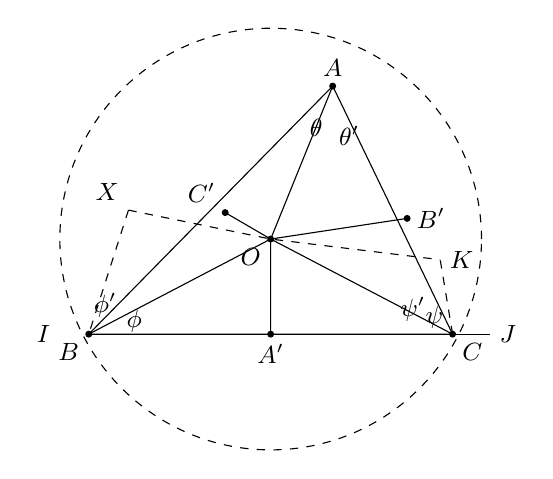
\begin{tikzpicture}[scale=1.05, every node/.style={font=\small}]
\coordinate (O) at (0,0);
\coordinate (B) at (-2.2,-1.15);
\coordinate (C) at (2.2,-1.15);
\coordinate (A) at (0.75,1.85);
\coordinate (Ap) at (0,-1.15);
\coordinate (Bp) at (1.65,0.25);
\coordinate (Cp) at (-0.55,0.32);
\coordinate (I) at (-2.55,-1.15);
\coordinate (J) at (2.65,-1.15);
\coordinate (K) at (2.05,-0.25);
\coordinate (X) at (-1.72,0.35);
\draw[dashed] (O) circle (2.55);
\draw (A)--(B)--(C)--cycle;
\draw (B)--(J);
\draw (O)--(A) (O)--(B) (O)--(C) (O)--(Ap) (O)--(Bp) (O)--(Cp);
\draw[dashed] (X)--(O)--(K);
\draw[dashed] (X)--(B);
\draw[dashed] (C)--(K);
\fill (O) circle (1.2pt) node[below left]{$O$};
\fill (A) circle (1.2pt) node[above]{$A$};
\fill (B) circle (1.2pt) node[below left]{$B$};
\fill (C) circle (1.2pt) node[below right]{$C$};
\fill (Ap) circle (1.2pt) node[below]{$A'$};
\fill (Bp) circle (1.2pt) node[right]{$B'$};
\fill (Cp) circle (1.2pt) node[above left]{$C'$};
\node at (I) [left] {$I$};
\node at (J) [right] {$J$};
\node at (K) [right] {$K$};
\node at (X) [above left] {$X$};
\node at (0.55,1.35) {$\theta$};
\node at (0.95,1.25) {$\theta'$};
\node at (-2.0,-0.8) {$\phi'$};
\node at (-1.65,-1.0) {$\phi$};
\node at (1.72,-0.85) {$\psi'$};
\node at (1.98,-0.95) {$\psi$};
\end{tikzpicture}
\end{center}

The radius of the absolute is for convenience taken to be $=1$; the distance of any
point from the centre can therefore be represented as the sine of an angle.

\pagemarker{410}{528}{474}

The distance $BC$, or say $\bar a$, of any two points $B,C$ is by definition as follows:
\[
\begin{array}{rl}
\hbox{Radius of circle}&=1,\\
\hbox{in }\triangle ABC,\ \hbox{sides are}&a,b,c,\\
\hbox{angles}&A,B,C,\\
OA,OB,OC&=\sin p,\sin q,\sin r,\\
OA',OB',OC'&=\sin a,\sin b,\sin c,\\
\angle BOC,\angle COA,\angle AOB&=\alpha,\beta,\gamma.
\end{array}
\]
Where $I,J$ are the intersections of the line $BC$ with the circle,
\[
e^{\bar a}+e^{-\bar a},\quad\hbox{or}\quad
2\cosh\bar a=\frac{BI.CJ}{BJ.CI}+\frac{BJ.CI}{BI.CJ}
=\frac{BI.CJ+BJ.CI}{\sqrt{BI.BJ.CI.CJ}}.
\]
The numerator is
\[
BI(BJ-BC)+CI(BC+CJ)=BI.BJ+CI.CJ+BC(CI-BI)=BI.BJ+CI.CJ+BC^2.
\]
Hence taking $a$ for the distance $BC$, and $\sin q,\sin r$ for the distances
$OB,OC$ respectively, we have $BI.BJ=\cos^2q$, $CI.CJ=\cos^2r$; and the formula is
\[
\cosh\bar a=\frac{\cos^2q+\cos^2r+a^2}{2\cos q\cos r}.
\]
Or, what is the same thing, taking $\alpha$ for the angle $BOC$, and therefore
\[
a^2=\sin^2q+\sin^2r-2\sin q\sin r\cos\alpha,
\]
we have
\[
\cosh\bar a=\frac{1-\sin q\sin r\cos\alpha}{\cos q\cos r}.
\]
In a similar manner, if $\sin a$ is the perpendicular distance from $O$ on the line
$BC$ (that is, $a\sin a=\sin q\sin r\sin\alpha$), it can be shown that
\[
\sinh\bar a=\frac{a\cos a}{\cos q\cos r},
\]
the equivalence of the two formulae appearing from the identity
\[
\cos^2q\cos^2r=(1-\sin q\sin r\cos\alpha)^2-a^2+a^2\sin^2a,
\]
which is at once verified.

Next for an angle; we have by definition
\[
\bar A=\frac1{2i}\log\frac{\sin BAI.\sin CAJ}{\sin BAJ.\sin CAI}.
\]

\pagemarker{411}{528}{475}

Where $AI,AJ$ are the (imaginary) tangents from $A$ to the circle; or writing for
shortness $BI$ \&c. instead of $BAI$ \&c. (the angular point being always at $A$),
\[
\bar A=\frac1{2i}\log\frac{\sin BI\,\sin CJ}{\sin BJ\,\sin CI}.
\]
Consequently
\[
e^{i\bar A}-e^{-i\bar A}
=2i\sin\bar A
=\frac{\sin BI\sin CJ-\sin BJ\sin CI}
{\sqrt{\sin BI\sin CJ}\sqrt{\sin BJ\sin CI}},
\]
where the numerator is
\[
\sin BI\sin(CJ-BC)-\sin CJ\sin(BI+BC)=\sin BC\sin IJ,
\]
or say $=\sin A\sin IJ$. Moreover taking the distance $OA$ to be $=\sin p$, and the
perpendicular distances from $O$ on the lines $AB,AC$ to be $\sin c$ and $\sin b$
respectively, then if for a moment the angle $IJ$ is put $=2\omega$, we have
$\sin p\sin\omega=1$; moreover
\[
\sin BI\sin BJ=\sin(\omega-BO)\sin(\omega+BO)=\sin^2\omega-\sin^2BO,
\]
and $\sin p\sin BO=\sin c$; that is,
\[
\sin BI\sin BJ=\frac{\cos^2c}{\sin^2p},
\qquad
\sin CI\sin CJ=\frac{\cos^2b}{\sin^2p}.
\]
Also
\[
\sin IJ=-\sin2\omega=2\sin\omega\cos\omega
=\frac{2\cos p}{\sin^2p}.
\]
Whence the required formula
\[
\sin\bar A=\frac{\cos p\sin A}{\cos b\cos c}.
\]
In the same way, or analytically from this value, we have
\[
\cos\bar A=\frac{\cos A+\sin b\sin c}{\cos b\cos c},
\]
and thence also
\[
\tan\bar A=\frac{\cos p\sin A}{\cos A+\sin b\sin c}.
\]
In particular, taking the line $AC$ to pass through $O$, or writing in the formula
$b=0$, we have
\[
BO=\tan^{-1}(\cos p\tan\theta),\qquad
CO=\tan^{-1}(\cos p\tan\theta');
\]
we ought to have
\[
A=BO+CO=\tan^{-1}(\cos p\tan\theta)+\tan^{-1}(\cos p\tan\theta'),
\]
which, observing that $\sin p\sin\theta=\sin c$ and $\sin p\sin\theta'=\sin b$, also
$A=\theta+\theta'$, is in fact equivalent to the above formula for $\tan\bar A$.
Observe in particular that when $A$ is at the centre, $p=0$, and the formula becomes
$\bar A=\theta+\theta'=A$, or say for an angle at the centre, $\bar A=A$.

\pagemarker{412}{528}{476}

I return to the expression for $\cosh\bar a$; in explanation of its meaning, let the
distances $OB,OC$ be $q,r$ respectively and let the angle $BOC$ be $\alpha$; to find
$\bar q$ we have only to take $C$ at $O$, that is, in the formula for $\cosh\bar a$ to
write $r=0$, we thus find
\[
\cosh\bar q=\frac1{\cos q},\qquad
\cosh\bar r=\frac1{\cos r},
\]
whence also
\[
\cos q=\sech\bar q,\quad \sin q=i\tanh\bar q,\qquad
\cos r=\sech\bar r,\quad \sin r=i\tanh\bar r.
\]
Also, as seen above, $\alpha=\alpha$; the formula thus is
\[
\begin{aligned}
\cosh\bar a
&=\frac{1+\tanh\bar q\,\tanh\bar r\cos\alpha}
{\sech\bar q\,\sech\bar r}\\
&=\cosh\bar q\cosh\bar r+\sinh\bar q\sinh\bar r\cos\alpha,
\end{aligned}
\]
or, what is the same thing, it is
\[
\cos\alpha=\frac{\cosh\bar a-\cosh\bar q\cosh\bar r}
{\sinh\bar q\sinh\bar r},
\]
viz. as will presently appear, this is the formula for $\cos BOC$ in the triangle
$BOC$.

From the above formulae
\[
\cosh\bar a=\frac{1-\sin q\sin r\cos\alpha}{\cos q\cos r},
\]
and
\[
\sin\bar A=\frac{\cos p\sin A}{\cos b\cos c},\qquad
\cos\bar A=\frac{\cos A+\sin b\sin c}{\cos b\cos c},
\]
and the like formulae for $b,c,B,C$, it may be shown that in the triangle $ABC$ we
have
\[
\cosh\bar a=\frac{\cos\bar A+\cos\bar B\cos\bar C}{\sin\bar B\sin\bar C}.
\]
In fact, substituting the foregoing values, this equation becomes
\[
\frac{(1-\sin^2a)(\cos A+\sin b\sin c)
+(\cos B+\sin c\sin a)(\cos C+\sin a\sin b)}
{\sin B\sin C\cos b\cos c}
=\frac{1-\sin q\sin r\cos\alpha}{\cos q\cos r},
\]
that is,
\[
\begin{aligned}
&\cos A+\cos B\cos C-\sin^2a\cos A+\sin a\sin b\cos B\\
&\quad+\sin a\sin c\cos C+\sin b\sin c
=\sin B\sin C(1-\sin q\sin r\cos\alpha),
\end{aligned}
\]
or, what is the same thing,
\[
\begin{aligned}
&\sin^2a(\cos B\cos C-\sin B\sin C)+\sin a\sin b\cos B\\
&\quad+\sin a\sin c\cos C+\sin b\sin c
=-\sin B\sin C\sin q\sin r\cos\alpha,
\end{aligned}
\]
that is,
\[
(\sin a\cos B+\sin c)(\sin a\cos C+\sin b)
=\sin B\sin C(\sin^2a-\sin q\sin r\cos\alpha),
\]
a relation which I proceed to verify.

\pagemarker{413}{528}{477}

We may, from the formulae
\[
a^2=\sin^2q+\sin^2r-2\sin q\sin r\cos\alpha,\qquad
a\sin a=\sin q\sin r\sin\alpha,\quad\hbox{\&c.},
\]
but, more simply, geometrically as presently shown, deduce
\[
\sin a\cos B+\sin c=a^{-1}\sin B\sin q(\sin q-\sin r\cos\alpha),
\]
\[
\sin a\cos C+\sin b=a^{-1}\sin C\sin r(\sin r-\sin q\cos\alpha),
\]
and thence
\[
\begin{aligned}
&(\sin a\cos B+\sin c)(\sin a\cos C+\sin b)\\
&\quad=a^{-2}\sin B\sin C\sin q\sin r
\{\sin q\sin r(1+\cos^2\alpha)-\cos\alpha(\sin^2q+\sin^2r)\}\\
&\quad=\sin B\sin C(\sin^2a-\sin q\sin r\cos\alpha),
\end{aligned}
\]
which is the equation in question. For the subsidiary equations used in the
demonstration, observe that the four points $O,X,A',B$ lie in a circle, and consequently
that
\[
CO.CX=CA'.CB;
\]
or multiplying each side by $\sin C$, then
\[
CO.CX.\sin C=A'K.CB,
\]
that is,
\[
\sin r(\sin r-\sin q\cos\alpha)\sin C
=a(\sin a\cos C+\sin b),
\]
and the other of the equations in question is proved in the same manner.

From the formula for $\cosh\bar a$ we find
\[
\sinh\bar a=\frac{\Delta}{\sin B\sin C},
\]
where
\[
\Delta^2=-(1-\cos^2A-\cos^2B-\cos^2C-2\cos A\cos B\cos C),
\]
whence also
\[
\sinh\bar a:\sinh\bar b:\sinh\bar c=\sin A:\sin B:\sin C;
\]
and we can also obtain
\[
\cos\bar A=\frac{\cosh\bar a-\cosh\bar b\cosh\bar c}
{\sinh\bar b\sinh\bar c}.
\]
So that the formulae are in fact similar to those of spherical trigonometry with only
$\cosh\bar a,\sinh\bar a$ \&c. instead of $\cos a,\sin a$ \&c. The before-mentioned
formula for $\cos\alpha$ in terms of $\bar a,\bar q,\bar r$ is obviously a particular case
of the last-mentioned formula for $\cos\bar A$.

\noindent\textit{Cambridge, 11 May, 1872.}

\clearpage
\section*{[529] A ``Smith's Prize'' Paper; Solutions}
\begin{center}
\textit{[From the Oxford, Cambridge and Dublin Messenger of Mathematics, vol. IV. (1868), pp. 201--226.]}
\end{center}

\pagemarker{414}{529}{478}

\textbf{1.} \textit{Find the form of a function of a given number of letters, which has two and only two values.}

It is required to find the general form of a function
$\phi(a,b,c,\ldots,k)$, rational and integral, which for all permutations whatever of
the letters has two and only two values.

Suppose that any particular permutation of the letters changes
$\phi(a,b,c,\ldots,k)$ into $\phi_1(a,b,c,\ldots,k)$; then any permutation of the letters
will either leave the functions $\phi,\phi_1$ each of them unaltered, or it will change
$\phi$ into $\phi_1$, and $\phi_1$ into $\phi$. Hence $\phi+\phi_1$ is a symmetrical function
of all the letters, say
\[
\phi+\phi_1=2L;
\]
$\phi-\phi_1$ is a function which by any permutation of the letters is either unaltered,
or simply changes its sign; and it is to be shown that, writing for shortness $V$ to
denote the product
\[
(a-b)(a-c)\cdots(b-c)\cdots
\]
of the differences of the letters, and denoting by $2M$ a symmetrical function of the
letters, we have
\[
\phi-\phi_1=2VM.
\]
These equations give
\[
\phi=L+VM,
\]
which is the general form required; viz. the function $\phi$ has then only the two
values $L+VM,L-VM$.

To prove the subsidiary theorem, observe that there is at least one interchange of two
letters which changes $\phi-\phi_1$ (for otherwise $\phi-\phi_1$ would be a symmetrical
function).\footnote{Set by me, for the Master of Trinity, Thursday, January 30, 1868.}

\pagemarker{415}{529}{479}

Let this be $(a,b)$. Then $\phi-\phi_1$, changing its sign for the interchange in
question, must vanish for $a=b$, that is, $\phi-\phi_1$ must contain the factor $(a-b)$;
let it contain it in the power $(a-b)^s$; then the quotient
$\phi-\phi_1\div(a-b)^s$, not vanishing for $a=b$, cannot change its sign by the
interchange in question, and as by supposition $\phi-\phi_1$ does change its sign, it
appears that the exponent $s$ must be odd. But $\phi-\phi_1$, containing the factor
$(a-b)^s$, must contain every other like factor $(a-c)^s$ or $(c-d)^s$; in fact,
writing $\phi-\phi_1=K(a-b)^s$, then if the interchange $(a,c)$ alters $K$ into $K_1$,
we have
\[
K(a-b)^s=\pm K_1(a-c)^s;
\]
and $K$ consequently contains the factor $(a-c)^s$; it does not contain any higher
power $(a-c)^{s+s'}$, for if it did, by reversing the process it would appear that
$\phi-\phi_1$ contained (contrary to supposition) the factor $(a-b)^{s+s'}$. Similarly
$\phi-\phi_1$ contains the factor $(c-d)^s$, but no higher power $(c-d)^{s+s'}$.
Hence $\phi-\phi_1$ contains the product of all the factors $(a-b)^s$, that is, it
contains $V^s$, and writing
\[
\phi-\phi_1=2V^sM,
\]
the quotient $M$ does not contain any such factor as $(a-b)$; it therefore does not
change its sign for any interchange whatever $(a,b)$; and in consequence it remains
unaltered for any such interchange, that is, $M$ is a symmetrical function. Observing
that any even power of $V$ is a symmetrical function, we may without loss of
generality include $V^{s-1}$ in the symmetrical function $M$, and write therefore
\[
\phi-\phi_1=2VM,
\]
which is the subsidiary theorem in question.

\textbf{2.} \textit{Express $\dfrac{x^7-1}{x-1}$ as the product of two cubic factors; and show
generally that, for any prime exponent $p$, the function $\dfrac{x^p-1}{x-1}$ may be
broken up into two factors each of the order $\frac12(p-1)$, by means of a quadratic
equation.}

Let $r$ be any root of the given equation, then
\[
r^6+r^5+r^4+r^3+r^2+r+1=0;
\]
the roots of this equation are $r^1,r^2,r^3,r^4,r^5,r^6$. Hence
\[
x^6+x^5+x^4+x^3+x^2+x+1
=(x-r^1)(x-r^2)(x-r^4)(x-r^3)(x-r^5)(x-r^6),
\]
and denoting the two cubic factors by $y_1,y_2$, or writing
\[
y_1=(x-r^1)(x-r^2)(x-r^4),\qquad
y_2=(x-r^3)(x-r^5)(x-r^6),
\]
we have
\[
\begin{aligned}
y_1&=x^3-x^2(r^1+r^2+r^4)+x(r^3+r^5+r^6)-1,\\
y_2&=x^3-x^2(r^3+r^5+r^6)+x(r^1+r^2+r^4)-1,
\end{aligned}
\]
and thence
\[
y_1+y_2=2x^3+x^2-x-2.
\]
Hence $y_1,y_2$ are the roots of the quadratic equation
\[
y^2-y(2x^3+x^2-x-2)+x^6+x^5+x^4+x^3+x^2+x+1=0.
\]

\pagemarker{416}{529}{480}

Solving the equation, observing that the quantity under the radical sign must of
necessity be a square, and that its value is
\[
(2x^3+x^2-x-2)^2-4(x^6+x^5+x^4+x^3+x^2+x+1),
\]
which is in fact
\[
=-7(x^2+x)^2,
\]
we find that the roots $y_1,y_2$, that is, the required cubic factors, are
\[
\frac12\{2x^3+x^2-x-2\pm\sqrt{-7}\,(x^2+x)\}.
\]
Generally for any prime exponent $p$, denoting any root by $r$, and writing
\[
y_1=(x-r^{a_1})(x-r^{a_2})\cdots,\qquad
y_2=(x-r^{b_1})(x-r^{b_2})\cdots,
\]
where $a_1,a_2,\ldots$ are the quadratic residues, and $b_1,b_2,\ldots$ the quadratic
non-residues of $p$, we find
\[
y^2-yP+Q=0,
\]
where $P$ is a function of $x$ of the order $\frac12(p-1)$, and
\[
Q=x^{p-1}+x^{p-2}+\cdots+x+1.
\]
Hence
\[
y=\frac12\{P\pm\sqrt{P^2-4Q}\},
\]
where $P^2-4Q$ is a perfect square, $=\eps pZ^2$, $Z$ a rational function of a degree
less than $\frac12(p-1)$, and $\eps=+$ or $-$ according as $p\equiv1$ or $\equiv3
\pmod 4$. Hence the required factors are
\[
\frac12\{P\pm\sqrt{\eps p}\,Z\}.
\]

\textbf{3.} \textit{In a Map of the World, wherein the meridians are projected into right
lines meeting in a point, the inclination of any two of the lines being equal to that
of the two meridians, and the parallels into circles about the point as centre, the
radius of the circle being a given function of the colatitude: compare on the sphere
and in the map (1) the corresponding elements of area, (2) the azimuths of
corresponding linear elements; and explain what conveniences may be obtained by
proper determinations of the above-mentioned function of the colatitude.}

Let the longitude and colatitude be
\[
\hbox{on the sphere }l,c,\qquad
\hbox{in the map }l',c',
\]
then the projection is such, that $l'=l$, $c'=f(c)$, a given function of $c$.
The lengths of corresponding linear elements in the direction of a meridian, and
perpendicular to it, are
\[
\dd c,\quad \sin c\,\dd l,
\]
\[
\dd c',\quad c'\dd l.
\]

\end{document}
